\subsection{可度量化空间的商空间}

若 X 是可度量化空间，R 是 X 上的一个等价关系，则商空间 X/R 未必可度量化（即使 X 局部紧 * 且 X/R 正规 * 也是如此）。然而：

命题 17. 紧可度量化空间的每个豪斯多夫商空间都是紧且可度量化的。

等价地，若 \(f\) 是紧可度量化空间 \(\mathbf{X}\) 到豪斯多夫空间 \(\mathbf{X}'\) 中的连续映射，则 \(f(\mathbf{X})\) 是 \(\mathbf{X}'\) 的可度量化子空间（第 I 章，§ 9，第 4 号，定理 2 的推论 4）。

设 \(\mathbf{X}\) 是紧可度量化空间，\(\mathbf{R}\) 是 \(\mathbf{X}\) 上的一个使 \(\mathbf{X} / \mathbf{R}\) 为豪斯多夫空间的等价关系。则 \(\mathbf{X} / \mathbf{R}\) 是紧的（第 I 章，§ 9，第 4 号，定理 2），故由命题 16，只需证明 \(\mathbf{X} / \mathbf{R}\) 的拓扑具有可数基。为此，我们要用到如下事实：\(\mathbf{R}\) 是闭的（第 I 章，§ 10，第 4 号，命题 8），并且模 \(\mathbf{R}\) 的各个等价类都是紧的。设 \(\varphi\) 是 \(\mathbf{X}\) 到 \(\mathbf{X} / \mathbf{R}\) 上的典范映射，\((\mathrm{U}_n)\) 是 \(\mathbf{X}\) 的拓扑的一个可数基。设 \(z\) 是 \(\mathbf{X} / \mathbf{R}\) 的任意一点，\(\mathbf{V}\) 是 \(z\) 在 \(\mathbf{X} / \mathbf{R}\) 中的一个邻域；则 \(\overline{\varphi}^1 (\mathbf{V})\) 是 \(\mathbf{X}\) 中紧集 \(\overline{\varphi}^1 (z)\) 的邻域。若 \(x\) 是 \(\overline{\varphi}^1 (z)\) 的任意一点，则存在一个集 \(\mathrm{U}_n\) ，它包含 \(x\) 且含于 \(\overline{\varphi}^1 (\mathrm{V})\) ；于是由波莱尔–勒贝格公理，存在一个有限开覆盖 \((\mathrm{U}_{n_k})_{1\leqslant k\leqslant r}\) ，它覆盖 \(\overline{\varphi}^1 (z)\) ，且使得：若以 \(\mathbf{W}\) 表示 \(\bigcup_{k}\mathrm{U}_{n_k},\mathrm{W}\) ，则它是 \(\overline{\varphi}^1 (z)\) 的一个含于 \(\overline{\varphi}^1 (\mathrm{V})\) 的邻域。由于 \(\mathbf{R}\) 是闭的，由此推出 \(\varphi (\mathbf{W})\) 是 \(z\) 在 \(\mathbf{X} / \mathbf{R}\) 中的一个含于 \(\mathbf{V}\) 的邻域（第 I 章，§ 5，第 4 号，命题 10）。设 \(\mathfrak{B}\) 表示形如 \(\varphi (\mathbf{W})\) 的集的内部所成的集，其中 \(\mathbf{W}\) 取遍集 \(\mathfrak{F}\) ，即形如 \(U_{n}\) 的集的一切有限并所成的集；这样我们便证明了 B 是 X/R 的拓扑的一个基，又因 F 是可数的，故 B 也是可数的。

命题 18. 设 X 是完备度量空间，R 是 X 上使 X/R 为豪斯多夫空间的开等价关系，\(\varphi: X \to X/R\) 是典范映射。则对 X/R 的任一紧子集 K，存在 X 的一个紧子集 \(K'\) 使 \(\varphi(K') = K\) 。

设 \(\mathfrak{B}_1\) 是 X 中以 \(1/2\) 为半径的全体开球所成的集。当 B 取遍 \(\mathfrak{B}_1\) 时，诸集 \(\varphi(B)\) 构成 K 的一个开覆盖，因此存在 X 的有限多个点 \(x_1, \ldots, x_m\) ，使得 \(\varphi\) 把以 \(1/2\) 为半径、以 \(x_i\) （ \(1 \leqslant i \leqslant m\) ）为中心的诸开球映为构成 K 的一个开覆盖的诸集。令 \(H_1 = \{x_1, \ldots, x_m\}\) ，并设已定义了有限集 \(H_i\) （ \(1 < i \leqslant n\) ），使得：

\begin{enumerate}
\def\labelenumi{(\roman{enumi})}
\item
  \(\mathbf{H}_i\subset \mathbf{H}_{i + 1}\) ，且 \(\mathbf{H}_{i + 1}\) 的每一点都以 \(<  \mathrm{I} / 2^{i}\) 的距离靠近 \(\mathbf{H}_i\) ，这里 \(\mathbf{I}\leqslant i\leqslant n - \mathbf{I};\)
\item
  \(\varphi\) 把以 \(1/2^i\) 为半径、以 \(\mathbf{H}_i\) 的点为中心的诸开球映为构成 \(\mathbf{K}\) 的开覆盖的诸开集，这里 \(1 \leqslant i \leqslant n\) 。
\end{enumerate}

设 \(\mathfrak{B}_{n+1}\) 是以 \(1/2^{n+1}\) 为半径、中心 \(x\) 满足 \(d(x, H_n) < 1/2^n\) （ \(d\) 为 X 上的度量）的全体开球所成的集。\(H_n\) 的性质表明，诸集 \(\varphi(B)\) （ \(B \in \mathfrak{B}_{n+1}\) ）构成 K 的开覆盖；因而存在有限集 \(L_{n+1} \subset X\) ，使得 \(\varphi\) 把以 \(1/2^{n+1}\) 为半径、中心属于 \(L_{n+1}\) 的诸开球映为构成 K 的一个开覆盖的诸集。取 \(H_{n+1} = H_n \cup L_{n+1}\) ，便知可以归纳地定义一个由 X 的有限子集组成的无限序列 \((H_n)\) ，它具有上述性质 (i) 与 (ii)。令 \(H = \bigcup_{n} H_n\) ，我们来证明 H 是预紧的。对每个 \(p > 0\) 及每点 \(z_{n+p} \in H_{n+p}\) ，存在点列 \(z_{n+i} \in H_{n+i}\) （ \(0 \leqslant i \leqslant p - 1\) ）使得

\[
d \left(z _ {n + i}, z _ {n + i + 1}\right) <   \mathrm{I} / 2 ^ {n + i} \quad \text { for } \quad \mathrm{o} \leqslant i \leqslant p - \mathrm{I};
\]

由此推出 \(d(z_n, z_{n+p}) \leqslant \sum_{i=0}^{p-1} \mathrm{I}/2^{n+i} \leqslant \mathrm{I}/2^{n-1}\) ，从而 \(d(y, \mathbf{H}_n) \leqslant \mathrm{I}/2^{n-1}\) 对一切 \(y \in \mathbf{H}\) 成立，这就证明了我们的断言。由于 \(\mathbf{X}\) 完备，\(\overline{\mathbf{H}}\) 是紧的，故 \(\varphi(\overline{\mathbf{H}})\) 是紧的。其次，我们证明 \(\mathbf{K} \subset \varphi(\overline{\mathbf{H}})\) 。若 \(z \in \mathbf{K}\) ，则按定义有 \(d(\overline{\mathbf{H}}_n, \overline{\varphi}^1(z)) \leqslant \mathrm{I}/2^n\) （对一切 \(n\) ），因而 \(d(\overline{\mathbf{H}}, \overline{\varphi}^1(z)) = 0\) ；但 \(\overline{\varphi}^1(z)\) 是闭集而 \(\overline{\mathbf{H}}\) 是紧集，故由此推出 \(\overline{\mathbf{H}} \cap \overline{\varphi}^1(z) \neq \emptyset\) （第 2 号，命题 3 后的注）；断言得证。于是，若 \(\mathbf{K}' = \overline{\mathbf{H}} \cap \overline{\varphi}^1(\mathbf{K})\) ，则 \(\mathbf{K}'\) 在 \(\overline{\mathbf{H}}\) 中闭，从而是紧的，并且由已证的结果有 \(\varphi(\mathbf{K}') = \mathbf{K}\) 。证毕。

\section{可度量化群、赋值域、赋范空间与赋范代数}

\subsection{可度量化拓扑群}

命题 1. 拓扑群 G 的左一致结构与右一致结构都可度量化，当且仅当 G 是豪斯多夫的且 G 的单位元 e 具有可数的基本邻域系。

该条件显然是必要的。反之，设它成立，令 \((\mathbf{V}_{n})\) 是 e 的一个基本邻域系；若以 \(U_{n}\) 表示诸对 \((x, y) \in \mathbf{G} \times \mathbf{G}\) 中满足 \(x^{-1}y \in V_{n}\) 者所成的集，则诸 \(U_{n}\) 构成 G 的左一致结构的一个可数围域基本系；由于此一致结构是豪斯多夫的，由 §2，第 4 号，定理 1 推出它是可度量化的。对 G 的右一致结构同理。

若拓扑群 G 的拓扑可度量化，则称 G 是可度量化的。于是命题 1 表明它的两个一致结构都是可度量化的。

借助下述概念，这一结果可以加强：

定义 1. 群 G（乘法记写）上的度量 d 称为左不变的（相应地，右不变的），如果我们有

\[
d (z x, z y) = d (x, y) \quad [ \text { resp. } d (x z, y z) = d (x, y) ]
\]

其中 \(x, y, z\) 取遍 \(\mathbf{G}\) 。

命题 2. 可度量化群 G 的左（相应地，右）一致结构可由 G 上的一个左不变（相应地，右不变）度量来定义。

设 e 的基本邻域系 \((\mathbf{V}_{n})\) 由对称邻域组成，使得 \(V_{n+1}^{3} \subset V_{n}\) 对每个 n 成立。~于是左一致结构的相应围域 \(U_{n}\) 是对称

的围域，且满足 \(\mathbf{U}_{n+1} \subset \mathbf{U}_n\) 。§1，第 4 号命题 2 的证明中所用的方法，使我们可以从围域序列 \((\mathbf{U}_n)\) 出发，构造出一个度量 \(d\) ，它定义在 \(\mathbf{G}\) 上且与 \(\mathbf{G}\) 的左一致结构相容；又因对每个 \(z \in \mathbf{G}\) ，映射 \((x, y) \to (zx, zy)\) 保持每个 \(\mathbf{U}_n\) 不变，由 \(d\) 的定义可知它是左不变度量。此方法对右一致结构同样适用。

注意，若 G 的两个一致结构不同，则度量 d 不是右不变的，因而一般地 \(d(x^{-1}, y^{-1}) \neq d(x, y)\) 。

特别地，若 G 是可度量化交换群，则它的一致结构由一个不变度量 d 定义；若 G 用加法记写，我们有

\[
d (x, y) = d (\mathrm{o}, y - x) = d (\mathrm{o}, x - y).
\]

我们常以 \(|x|\) （或 \(||x||\) ）表示 \(d(0, x)\) ；这时

\[
d (x, y) = | x - y |.
\]

函数 \(|x|\) 满足下列三个条件：

\begin{enumerate}
\def\labelenumi{\alph{enumi})}
\item
  \(|-x| = |x|\) 对一切 \(x \in G\) 成立。
\item
  \(|x + y| \leqslant |x| + |y|\) 对一切 \(x \in G\) 与一切 \(y \in G\) 成立。
\item
  \(|x| = 0\) 当且仅当 \(x = 0\) 。
\end{enumerate}

反之：

命题 3. 设 G 是用加法记写的交换群，\(x \to |x|\) 是满足上述条件 a)、b)、c) 的一个映射 \(\mathbf{G} \to \mathbf{R}_+\) 。则函数 \(d(x, y) = |x - y|\) 是 G 上的不变度量；它在 G 上定义的拓扑 C 与 G 的群结构相容，且由 d 定义的一致结构与赋有拓扑 C 的 G 所成拓扑群的一致结构相同。

函数 \(d(x, y)\) 是 \(G\) 上的度量，因为关系 \(d(x, y) = 0\) 等价于 \(x = y\) （由 \(c\) ）；而有 \(d(x, y) = d(y, x)\) （由 \(a\) ）；并且

\[
d (x, y) = | (x - z) + (z - y) | \leqslant | x - z | + | z - y | = d (x, z) + d (z, y)
\]

这是由 \(b\) ) 得到的。此外，\(d\) 是不变的，因为 \((x + z) - (y + z) = x - y\) 。对每个实数 \(\alpha > 0\) ，令 \(V_{\alpha}\) 为全体 \(x \in G\) 中满足 \(|x| < \alpha\) 者所成的集；则诸 \(V_{\alpha}\) 构成一个基本邻域系 \(\mathfrak{S}\) ，即 \(o\) 关于拓扑 \(\mathfrak{C}\) 的基本邻域系；又因 \(d\) 不变，\(a + \mathfrak{S}\) 是 \(a\) 的一个基本邻域系（关于拓扑 \(\mathfrak{C}\) ；这里 \(a \in G\) 任意）。由 \(a\) ，诸 \(V_{\alpha}\) 是对称的；由 \(b\) ，有 \(V_{\alpha} + V_{\alpha} \subset V_{2\alpha}\) ；因而拓扑 \(\mathfrak{C}\) 与 \(G\) 的群结构相容（第 III 章，§ 1，第 2 号）。命题的最后一部分立即可得。

条件 \(a), b)\) 与 \(c)\) 等价于 \(c)\) 连同条件

\[
| x - y | \leqslant | x | + | y |.\tag{\(b^{\prime}\)}
\]

因为 \(a)\) 与 \(b)\) 显然蕴含 \(b')\) ；反之，取 \(x = 0\) 代入 \(b')\) 并利用 \(c)\) ，得 \(|-y| \leqslant |y|\) ；把 \(y\) 换成 \(-y\) 便得 \(|-y| = |y|\) ，此即 \(a)\) ；再把 \(y\) 换成 \(-y\) 代入 \(b')\) 即得 \(b)\) 。

命题 4. 若 G 是可度量化群，则 G 的每个豪斯多夫商群 G/H 都可度量化。若 G 还是完备的，则 G/H 是完备的 (*)。

命题的第一部分是如下事实的推论：G/H 的单位元在 G/H 中具有可数的基本邻域系；因为若 \((\mathbf{V}_{n})\) 是 e 在 G 中的基本邻域系，则 \(\dot{V}_{n}\) （诸集 \(V_{n}\) 在 G/H 中的典范像）构成 G/H 的单位元的基本邻域系（第 III 章，§ 2，第 6 号，命题 17）。

要证明当 G 完备时 G/H 也完备，由 § 2，第 6 号，命题 9，只需证明每个柯西序列 \((\dot{x}_{n})\) （关于 G/H 的左一致结构）都收敛。必要时可代之以 \((\dot{x}_{n})\) 的子序列，从而可设对每对满足 \(p \geqslant n\) 且 \(q \geqslant n\) 的指标 p、q，有 \(\dot{x}_{p}^{-1}\dot{x}_{q} \in \dot{V}_{n}\) ；这表示对每对点 \(y \in \dot{x}_{p}, z \in \dot{x}_{q}\) ，有 \(y^{-1}z \in HV_{n} = V_{n}H\) ；因而对每个 \(y \in \dot{x}_{p}\) ，\(\dot{x}_{q}\) 与 y 的邻域 \(yV_{n}\) 之交非空。现设序列 \((V_{n})\) 已选得使 \(V_{n+1}^{2} \subset V_{n}\) ，并归纳地定义 G 中点的序列 \((x_{n})\) ，使得 \(x_{n} \in \dot{x}_{n}\) 且 \(x_{n+1} \in x_{n}V_{n}\) ；由前所述这是可能的。于是由归纳法推出，对每个 p \textgreater{} 0 有 \(x_{n+p} \in x_{n}V_{n}V_{n+1} \ldots V_{n+p-1} \subset x_{n}V_{n-1}\) 。因此序列 \((x_{n})\) 是 G 中的柯西序列，故收敛于一点 a；并且立即得出，a 在 G/H 中的典范像 \(\dot{a}\) 是序列 \((\dot{x}_{n})\) 的极限。

推论 1. 设 G 是完备可度量化群，\(G_{0}\) 是 G 的稠密子群，\(H_{0}\) 是 \(G_{0}\) 的闭正规子群。若 H 是 \(H_{0}\) 在 G 中的闭包，则商群 \(G_{0}/H_{0}\) 的完备化同构于 G/H。

H 是 G 的正规子群（第 III 章，§ 2，第 3 号，命题 8），且命题 4 表明 G/H 是完备的。又若 \(\varphi\) 是 G 到 G/H 上的典范映射，则显然 \(\varphi(G_0)\) 在 G/H 中稠密。因此结论由第 III 章，§ 2，第 7 号，命题 21 得出。

设 \(G, G'\) 是两个豪斯多夫交换拓扑群，\(\hat{G}, \hat{G}'\) 是它们各自的完备化。我们回忆（第 III 章，§ 3，第 3 号，命题 5）：若 \(u\) 是 \(G\) 到 \(G'\) 中的连续同态，则 \(u\) 一致连续，且可唯一扩张为 \(\hat{G}\) 到 \(\hat{G}'\) 中的连续同态 \(\hat{u}\) ，在以下

本小节的其余部分中即用此记号。图表

\pandocbounded{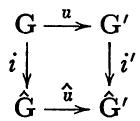
\includegraphics[keepaspectratio]{images/part001_945be03d.jpg}}

（其中 \(i\) ， \(i'\) 是典范单射）是交换的。若 \(v\) 是 \(\mathbf{G}'\) 到豪斯多夫交换拓扑群 \(\mathbf{G}''\) 中的连续同态，且 \(w = v \circ u\) ，则立即得出 \(\hat{w} = \hat{v} \circ \hat{u}\) 。

设 H 是 G 的闭子群，令 E = G/H。设 \(j: H \to G\) 与 \(p: G \to E\) 是典范映射。设 \(\overline{H}\) 是 H 在 \(\hat{G}\) 中的闭包；\(\overline{H}\) 是完备群，我们把它与 H 的完备化 \(\hat{H}\) 等同。j 的连续延拓 \(\hat{j}\) （到 \(\hat{H}\) 上）显然是 \(\hat{H}\) 到 \(\hat{G}\) 中的典范单射。

以下设 G 是可度量化的。于是 E = G/H 到 \(\hat{G}/\hat{H}\) 中的典范映射是 E 到完备群 \(\hat{G}/\hat{H}\) 的一个稠密子群上的拓扑同构（推论 1），从而我们可把 \(\hat{G}/\hat{H}\) 与 \(\hat{E}\) 等同，并把 p 的连续延拓 \(\hat{p}\) （到 \(\hat{G}\) 上）与 \(\hat{G}\) 到 \(\hat{G}/\hat{H}\) 上的典范映射等同。

推论 2. 设 G，G‘ 是两个可度量化交换拓扑群；u: G → G’ 是严格态射，其核为 N、像为 P。则 \(\hat{u} : \hat{G} \rightarrow \hat{G}'\) 是严格态射，其核为 \(\hat{N}\) 、像为 \(\hat{P}\) 。

设 \(u = j \circ v \circ p\) 是 \(u\) 的典范分解，其中 \(v\) 是拓扑群 \(G/N\) 到拓扑群 \(u(G) = P\) 上的同构。我们有 \(\hat{u} = \hat{j} \circ \hat{v} \circ \hat{p}\) ，并且已经看到 \(\hat{p}\) 是 \(\hat{G}\) 到 \(\hat{G}/\hat{N}\) 上的典范映射，而 \(\hat{j}\) 是 \(\hat{P}\) 到 \(\hat{G}'\) 中的典范映射。另一方面，\(\hat{v}\) 是 \(\hat{G}/\hat{N}\) 到 \(\hat{P}\) 上的同构（第 III 章，§ 3，第 4 号，命题 5），由此即得结论。

推论 3. 设 \(\mathbf{G}, \mathbf{G}'\) ， \(\mathbf{G}''\) 是三个可度量化交换拓扑群，\(u: \mathbf{G} \to \mathbf{G}'\) 与 \(v: \mathbf{G}' \to \mathbf{G}''\) 是两个严格态射，使得序列 \(\mathbf{G} \xrightarrow{u} \mathbf{G}' \xrightarrow{v} \mathbf{G}''\) 是正合的{[}即 \(u(\mathbf{G}) = \overline{v}^{1}(\mathbf{o})\) {]}。则序列 \(\hat{\mathbf{G}} \xrightarrow{\hat{u}} \hat{\mathbf{G}}' \xrightarrow{\hat{v}} \hat{\mathbf{G}}''\) 是正合的。

因为若令 \(\mathrm{N} = u(\mathrm{G}) = \overline{v}^{1}(\mathrm{o})\) ，则由推论 2，\(\hat{N}\) 既是 \(\hat{u}\) 的像又是 \(\hat{v}\) 的核。

注。1) 设 G 是非豪斯多夫拓扑群，但与之相伴的豪斯多夫群可度量化；等价地，G 的单位元在 G 中具有可数的基本邻域系。命题 4 的证明可不加修改地用于这一情形（H 为 G 的任意正规子群），它表明与 G/H 相伴的豪斯多夫群可度量化，并且只要 G 完备，G/H 就是完备群（一般不是豪斯多夫的）。

\begin{enumerate}
\def\labelenumi{\arabic{enumi})}
\setcounter{enumi}{1}
\tightlist
\item
  设 \(d\) 是定义可度量化群 G 的拓扑的左不变度量，H 是 G 的闭正规子群。若 \(\dot{x}\) 与 \(\dot{y}\) 是 G/H 的任意两点，考虑距离 \(d(\dot{x},\dot{y})\) ，即 G 中两个闭子集 \(\dot{x},\dot{y}\) 之间的距离（§ 2，第 2 号）；我们将看到，这个函数是 G/H 上的左不变度量，并且定义这个商群的拓扑。
\end{enumerate}

首先注意，若 \(x \in \dot{x}\) 且 \(y \in \dot{y}\) ，则有 \(d(\dot{x}, \dot{y}) = d(x, \mathrm{H}y)\) ；因为 \(d(x, \mathrm{H}y) = \inf_{h \in \mathbf{H}} d(x, h y)\) ，从而 \(d(h' x, \mathrm{H} y) = d(x, \mathrm{H} y)\) 对一切 \(h' \in \mathrm{H}\) 成立，因为 \(d\) 是左不变的；这就证明了断言（§ 2，第 2 号）。于是对每个 \(\dot{z} \in \mathrm{G} / \mathrm{H}\) 有{[}§ 2，第 2 号，公式 (2){]}

\[
\left| d (\dot {x}, \dot {z}) - d (\dot {y}, \dot {z}) \right| = \left| d (x, \dot {z}) - d (y, \dot {z}) \right| \leqslant d (x, y);
\]

又因这个不等式对一切 \(x \in \dot{x}\) 与一切 \(y \in \dot{y}\) 成立，我们有 \(|d(\dot{x}, \dot{z}) - d(\dot{y}, \dot{z})| \leqslant d(\dot{x}, \dot{y})\) ，这表明 \(d(\dot{x}, \dot{y})\) 是 G/H 上的度量。此外，对任意 \(z \in \dot{z}\) ，我们有

\[
d (\dot {z} \dot {x}, \dot {z} \dot {y}) = \inf _ {h \in \mathbf {H}} d (z x, h z y)
\]

这是由上面的式子得到的；但由于 \(hzy = z(z^{-1}hz)y\) ，并且 \(z^{-1}hz\) 随 \(h\) 取遍 H 而取遍 H（H 是正规的），\(d(x,y)\) 的左不变性表明有 \(d(zx, \mathrm{Hz}) = d(x, \mathrm{Hy}) = d(\dot{x}, \dot{y})\) 。最后，若 V 是 G 中 \(e\) 的由 \(d(e, x) < \alpha\) 定义的邻域，则 V 在 G/H 中的像 V 就是由 \(d(\dot{e}, \dot{x}) < \alpha\) 定义的集；这就完成了证明。

\subsection{赋值除环}

定义 2. 除环 K 上的绝对值是一个映射 \(x \to |x|\) ，它把 K 映入 \(\mathbf{R}_{+}\) ，且满足下列条件：

\((\mathbf{VM}_{\mathbf{I}})\) \(|x| = 0\) 当且仅当 \(x = 0\) 。

\((\mathbf{VM}_{\mathbf{II}})\quad |xy| = |x|.|y|\) 对一切 \(x,y\) （\(\mathbf{K}\) 中的）成立。

\((\mathbf{VM}_{\mathbf{III}})\quad |x + y|\leqslant |x| + |y|\) 对一切 \(x,y\) （\(\mathbf{K}\) 中的）成立。

由 \((\mathbf{VM}_{\mathbf{II}})\) 有 \(|x| = |\mathrm{I}|.|x|\) ，又由 \((\mathbf{VM}_{\mathbf{I}})\) 至少有一个 \(x\) 使 \(|x| \neq 0\) ，故 \(|\mathrm{I}| = \mathrm{I}\) ；由此推出 \(\mathrm{I} = |- \mathrm{I}|^2\) ，因此 \(|- \mathrm{I}| = \mathrm{I}\) ，从而

\[
| - x | = | - \mathrm{I} | | x | = | x |;
\]

因此 \(|x - y| \leqslant |x| + |y|\) 对一切 \(x, y\) （\(\mathbf{K}\) 中的）成立。于是我们可以说，\(d(x, y) = |x - y|\) 是加法群 \(\mathbf{K}\) 上的不变度量，并且映射 \(x \to |x|\) 是由 K 的非零元素组成的乘法群 \(K^{*}\) 到乘法群 \(R_{+}^{*}\) （由实数 \textgreater0 组成）中的同态。

不变度量 \(|x - y|\) 在 K 上定义了一个度量空间拓扑，它与 K 的加法群结构相容（第 1 号，命题 3）；而且，这一拓扑与 K 的除环结构相容。因为 xy 在 \(K \times K\) 上的连续性由关系式

\[
x y - x _ {0} y _ {0} = (x - x _ {0}) (y - y _ {0}) + (x - x _ {0}) y _ {0} + x _ {0} (y - y _ {0}),
\]

由此得到

\[
\left| x y - x _ {0} y _ {0} \right| \leqslant \left| x - x _ {0} \right|. \left| y - y _ {0} \right| + \left| x _ {0} \right|. \left| y - y _ {0} \right| + \left| y _ {0} \right|. \left| x - x _ {0} \right|.
\]

同样，\(x^{-1}\) 在每一点 \(x_{0} \neq 0\) 处的连续性由恒等式 \(x^{-1} - x_{0}^{-1} = x^{-1} (x_{0} - x)x_{0}^{-1}\) 得出，由 \((\mathrm{VM}_{\mathrm{II}})\) 它给出

\[
\left| x ^ {- 1} - x _ {0} ^ {- 1} \right| = \frac {\left| x - x _ {0} \right|}{\left| x _ {0} \right| . \left| x \right|};
\]

现若 \(\varepsilon > 0\) 满足 \(\varepsilon < |x_0|\) ，则关系 \(|x - x_0| \leqslant \varepsilon\) 蕴含 \(|x| \geqslant |x_0| - \varepsilon\) ，由此得 \(|x^{-1} - x_{0}^{-1}| \leqslant \varepsilon / |x_0| (|x_0| - \varepsilon)\) ；这就建立了 \(x^{-1}\) 在点 \(x_0\) 处的连续性。

定义 3. 赋值除环就是赋有由 K 上一个给定绝对值所定义之结构的除环 K。

赋值除环总被视为赋有由其绝对值定义的拓扑，这使它成为拓扑除环。若 \(K_{0}\) 是赋值除环 K 的一个子除环，则 K 上的绝对值在 \(K_{0}\) 上的限制是 \(K_{0}\) 上的一个绝对值，它在 \(K_{0}\) 上定义由 K 的拓扑诱导的拓扑。

例。1) 设 K 是任意除环。对每个 \(x \in \mathbf{K}\) ，令 \(|x| = \mathbf{i}\) （若 \(x \neq 0\) ），并令 \(|0| = 0\) 。如此定义的映射 \(x \to |x|\) 是 K 上的绝对值，称为平凡绝对值。除环 K 上由绝对值 \(|x|\) 定义的拓扑是离散的，当且仅当 \(|x|\) 是平凡绝对值。此条件显然是充分的；反之，若 K 的拓扑是离散的，则 \(|x|\) 不能取任何 \(\alpha > 0\) 的值，除非它是 \(\mathbf{i}\) ；因为若有 \(|x_0| = \alpha < \mathbf{i}\) ，则序列 \((x_0^n)\) 将由非零项组成且收敛于 \(\mathbf{o}\) ；要处理 \(\alpha > \mathbf{i}\) 的情形，就用 \(x_0^{-1}\) 代替 \(x_0\) 。

\begin{enumerate}
\def\labelenumi{\arabic{enumi})}
\setcounter{enumi}{1}
\item
  实数的绝对值（第 IV 章，§ 1，第 6 号）满足公理 \((\mathrm{VM}_{\mathrm{I}})\) ， \((\mathrm{VM}_{\mathrm{II}})\) 与 \((\mathrm{VM}_{\mathrm{III}})\) ，并且它在域 \(\mathbf{R}\) 上定义的拓扑就是实直线的拓扑。在复数域 \(\mathbf{C}\) （与 \(\mathbf{R}^2\) 等同）上{[}相应地，四元数体 \(\mathbf{H}\) （与 \(\mathbf{R}^4\) 等同）上{]}，欧氏范数同样是绝对值，并且定义域 C（相应地，除环 H）的拓扑（第 VIII 章，§ 1，第 2 号与第 4 号）。
\item
  在除环 K 上，实赋值是定义在 \(K^{*}\) 上、取值于 R 中的函数 v，它满足下列条件：a) 若 \(x \in K^{*}\) 且 \(y \in K^{*}\) ，则 \(v(xy) = v(x) + v(y)\) ；b) 若此外还有 \(x + y \neq 0\) ，则 \(v(x + y) \geqslant \inf(v(x), v(y))\) 。若 a 是任一实数 \textgreater1，则令 \(|x| = a^{-v(x)}\) （对 \(x \neq 0\) ），并令 \(|0| = 0\) ，便可在 K 上定义一个绝对值。因为关系式 \(v(xy) = v(x) + v(y)\) （对 \(x \neq 0\) 与 \(y \neq 0\) ）蕴含对这些 x、y 值的关系式 \(|xy| = |x|.|y|\) ，且当 x、y 之一为零时此关系平凡成立；同样，由关系式 \(v(x + y) \geqslant \inf(v(x), v(y))\) （当 \(x \neq 0\) 、 \(y \neq 0\) 且 \(x + y \neq 0\) 时）推出 \(|x + y| \leqslant \sup(|x|, |y|) \leqslant |x| + |y|\) ，并且当 x、y、 \(x + y\) 之一为零时这些不等式仍然成立。特别地，若 \(v_{p}(x)\) 是有理数域 Q 上的 p 进赋值（x 的素因子分解中 p 的指数），则相应的绝对值 \(|x|_{p} = p^{-v_{p}(x)}\) 称为域 Q 上的 p 进绝对值（参见第 III 章，§ 6，习题 23）。
\end{enumerate}

注。若 \(x\) 是赋值除环中的单位根，则 \(|x| = 1\) ，因为 \(x^n = 1\) 蕴含 \(|x|^n = 1\) ，从而 \(|x| = 1\) 。特别地，有限域上唯一的绝对值是平凡绝对值，因为这种域的每个元素 \(\neq 0\) 者都是单位根。

定义 4. 除环 K 上的两个绝对值称为等价的，如果它们在 K 上定义相同的拓扑。

命题 5. 两个绝对值 \(|x|_1, |x|_2\) （在除环 \(K\) 上，均非平凡绝对值）等价，当且仅当关系 \(|x|_1 < i\) 蕴含 \(|x|_2 < i\) 。这时存在实数 \(\rho > 0\) ，使得 \(|x|_2 = |x|_1^p\) 对一切 \(x \in K\) 成立。

此条件是必要的，因为全体 \(x \in \mathbf{K}\) 中满足 \(|x|_1 < 1\) 者所成的集，与全体 \(x\) 中关于由绝对值 \(|x|_1\) 定义的拓扑使 \(\lim x^n = 0\) 者所成的集相同。

反之，设 \(|x|_1 < \mathrm{i} \Longrightarrow |x|_2 < \mathrm{i}\) 。则有 \(|x|_1 > \mathrm{i} \Longrightarrow |x|_2 > \mathrm{i}\) ，因为 \(|x^{-1}|_1 < \mathrm{i}\) ，从而 \(|x^{-1}|_2 < \mathrm{i}\) 。由假设绝对值 \(|x|_1\) 不是平凡的，故存在 \(x_0 \in \mathbf{K}\) 使 \(|x_0|_1 > \mathrm{i}\) 。令 \(a = |x_0|_1\) ， \(b = |x_0|_2\) ，并令 \(\rho = \log b / \log a > 0\) 。设 \(x \in \mathbf{K}^*\) ，令 \(|x|_1 = |x_0|^{\gamma}\) 。若整数 \(m\) 与 \(n\) 满足 \(n > 0\) 且 \(m/n > \gamma\) ，则 \(|x|_1 < |x_0|_1^{m/n}\) ，因此 \(|x^n x_0^{-m}|_1 < \mathrm{i}\) ；于是 \(|x^n x_0^{-m}|_2 < \mathrm{i}\) ，即 \(|x|_2 < |x_0|_2^{m/n}\) 。类似地，若 \(m/n < \gamma\) ，则得 \(|x|_2 > |x_0|_2^{m/n}\) ；由此推出 \(|x|_2 = |x_0|_2^\gamma\) ；换言之

\[
\log | x | _ {2} = \gamma \log b = \gamma \rho \log a = \rho \log | x | _ {1},
\]

即 \(|x|_2 = |x|_1^p\) 。现在显然，在 \(\mathbf{K}\) 上由 \(|x|_1\) 与 \(|x|_2\) 定义的诸拓扑的零邻域是相同的。

反之，若 \(|x|\) 是 \(K\) 上任一绝对值，则函数 \(|x|^{\circ}\) 是 \(K\) 上的绝对值（与 \(|x|\) 等价），对一切 \(\rho\) （满足 \(0 < \rho \leqslant 1\) ）。只需验证不等式 \(|x + y|^{\circ} \leqslant |x|^{\circ} + |y|^{\circ}\) ；由于 \(|x + y|^{\circ} \leqslant (|x| + |y|)^{\circ}\) ，只需证明：若 \(a > 0\) 且 \(b > 0\) ，则 \((a + b)^{\circ} \leqslant a^{\circ} + b^{\circ}\) 对任何 \(\rho\) （满足 \(0 < \rho \leqslant 1\) ）成立。若令 \(c = a / (a + b)\) 与 \(d = b / (a + b)\) ，则有 \(c + d = 1\) ，待证的不等式为 \(c^{\circ} + d^{\circ} \geqslant 1\) ；但这由关系式 \(c^{\circ} \geqslant c\) 与 \(d^{\circ} \geqslant d\) 立即得出，它们当 \(0 < c \leqslant 1\) 、 \(0 < d \leqslant 1\) 、 \(0 < \rho \leqslant 1\) 时成立。

因此，r \textgreater{} 0 中使 \(|x|^{r}\) 成为绝对值的那些值的集合是 R 中以 o 为左端点的有限或无限区间；若它是有限的，则它显然是闭的；因为若 \(|x + y|^{r} \leqslant |x|^{r} + |y|^{r}\) 对 K 中任意 x、y 及一切满足 \(0 < r < r_{0}\) 的 r 成立，则由连续性该不等式对 \(r = r_{0}\) 仍成立。若 \(|x|^{r}\) 对一切 r \textgreater{} 0 都是绝对值，则我们有

\[
| x + y | \leqslant (| x | ^ {r} + | y | ^ {r}) ^ {1 / r}
\]

对一切 \(x\) 与 \(y\) （\(\mathbf{K}\) 中的）以及一切 \(r > 0\) 成立。现在，若 \(a, b\) 是两个实数 \(\geqslant 0\) ，则有 \(\lim_{r \to \infty} (a^r + b^r)^{1/c} = \sup (a, b)\) ；因为，例如设 \(a \geqslant b\) ，我们有 \(a \leqslant (a^r + b^r)^{1/r} \leqslant 2^{1/r} a\) ，令 \(r \to +\infty\) 即得结果。

于是，若 \(|x|^r\) 对一切 \(r > 0\) 是绝对值，则我们有

\[
| x + y | \leqslant \sup (| x |, | y |)
\]

这可以表述为：\(v(x) = -\log |x| (x \neq 0)\) 是 K 上的赋值。

注。命题 5 的证明表明：若由 \(|x|_2\) 定义的拓扑比由 \(|x|_1\) 定义的拓扑粗，且 \(|x|_1\) 不是平凡的，则 \(|x|_1\) 与 \(|x|_2\) 等价，因为这时关系 \(|x|_2 < 1\) 蕴含 \(|x|_2 < 1\) 。于是，\(K\) 上两个均非平凡的绝对值所定义的拓扑不能比较而不相同。

命题 6. 设 \(\hat{\mathbf{K}}\) 是除环 \(\mathbf{K}\) 赋有绝对值 \(|x|\) 后的完备化，则它是一个除环，且函数 \(|x|\) 可由连续性扩张为 \(\hat{\mathbf{K}}\) 上的绝对值，它定义 \(\hat{\mathbf{K}}\) 的拓扑。

设 \(\mathfrak{F}\) 是 K 上的柯西滤子（关于加法一致结构），它不以 o 为聚点；要证明 \(\hat{\mathbf{K}}\) 是除环，只需证明 \(\mathfrak{F}\) 在映射 \(x \to x^{-1}\) 下的像是柯西滤子基（第 III 章，§ 6，第 8 号，命题 7）。由假设，存在实数 \(\alpha > 0\) 与集 \(\mathrm{A} \in \mathfrak{F}\) ，使得 \(|x| \geqslant \alpha\) 对一切 \(x \in \mathrm{A}\) 成立；另一方面，对每个 \(\varepsilon > 0\) 存在集 \(\mathrm{B} \in \mathfrak{F}\) ，使得 \(\mathrm{B} \subset \mathrm{A}\) 且 \(|x - y| \leqslant \varepsilon\) 对一切 \(x \in \mathrm{B}\)

与 \(y\in \mathbf{B}\) 成立；由此

\[
\left| x ^ {- 1} - y ^ {- 1} \right| = \frac {\left| x - y \right|}{\left| x \right| . \left| y \right|} \leqslant \frac {\varepsilon}{\alpha^ {2}},
\]

这就得出命题的第一部分。不变度量 \(|x - y| = d(x, y)\) 由连续性扩张为 \(\hat{\mathbf{K}}\) 上的度量（§ 2，第 1 号，命题 1），它定义 \(\hat{\mathbf{K}}\) 的拓扑，且由恒等式延拓原理是不变的；我们仍以 \(d(x, y)\) 记这个不变度量。若令 \(|x| = d(0, x)\) （对 \(x \in \hat{\mathbf{K}}\) ），则显然 \(|x|\) 是函数 \(|x|\) （\(\mathbf{K}\) 上的）的连续延拓，从而由恒等式延拓原理是 \(\hat{\mathbf{K}}\) 上的绝对值。

\subsection{赋值除环上的赋范空间}

定义 5. 若 E 是非离散赋值除环 K 上的（左）向量空间，E 上的范数是一个映射 \(\mathbf{x} \to p(\mathbf{x})\) ，它把 E 映入 \(\mathbf{R}_+\) ，且满足下列公理：

\[
\left(\mathrm{NO} _ {\mathbf {I I}}\right) \quad p (\boldsymbol {x} + \boldsymbol {y}) \leqslant p (\boldsymbol {x}) + p (\boldsymbol {y}) \text {   for   all   } \boldsymbol {x}, \boldsymbol {y} \text {   in   } \mathbf {E};
\]

\[
\left(\mathrm{NO} _ {\mathbf {I I I}}\right) \quad p (t \boldsymbol {x}) = | t | p (\boldsymbol {x}) \text {for all} t \in \mathrm{K} \text {and all} \boldsymbol {x} \in \mathrm{E}.
\]

最常遇到的赋范空间以 R 或 C 为标量域（带通常绝对值）。

由 \((\mathrm{NO}_{\mathrm{III}})\) 特别推出 \(p(-x)=p(x)\) ；因此若令 \(d(x,y)=p(x-y)\) ，则 d 是加法群 E 上的不变度量，并且定义一个与 E 的加法群结构相容的度量空间拓扑（第 1 号，命题 3）；此外，映射

\[
(t, \boldsymbol {x}) \rightarrow t \boldsymbol {x}
\]

在 \(\mathbf{K} \times \mathbf{E}\) 上连续；因为我们有

\[
t \boldsymbol {x} - t _ {0} \boldsymbol {x} _ {0} = (t - t _ {0}) (\boldsymbol {x} - \boldsymbol {x} _ {0}) + (t - t _ {0}) \boldsymbol {x} + t _ {0} (\boldsymbol {x} - \boldsymbol {x} _ {0})
\]

由此得到

\[
p (t \boldsymbol {x} - t _ {0} \boldsymbol {x} _ {0}) \leqslant | t - t _ {0} | p (\boldsymbol {x} - \boldsymbol {x} _ {0}) + | t - t _ {0} | p (\boldsymbol {x}) + | t _ {0} | p (\boldsymbol {x} - \boldsymbol {x} _ {0}),
\]

这表明只要取 \(|t - t_{0}|\) 与 \(p(x - x_{0})\) 充分小，就可使左端任意小。

定义 6. 若 K 是非离散赋值除环，则 K 上的向量空间 E 赋有由 E 上一个给定范数所定义的结构后，称为 K 上的赋范空间。

赋范空间总被视为赋有由其范数定义的拓扑与一致结构。

例。1) 在非离散赋值除环 K 上，把 K 自身看作（左或右）向量空间，绝对值 \(|x|\) 是一个范数。

\begin{enumerate}
\def\labelenumi{\arabic{enumi})}
\setcounter{enumi}{1}
\item
  表达式 \(||x|| = \sqrt{\sum_{i=1}^{n} x_i^2}\) ——我们曾称之为空间 \(\mathbf{R}^n\) 上的欧氏范数（第 VI 章，§ 2）——显然是定义 5 意义下的范数。函数 \(\sup_{1 \leqslant i \leqslant n} |x_i|\) 与 \(\sum_{i=1}^{n} |x_i|\) 也是范数。
\item
  设 \(\mathcal{B}(\mathrm{E};\mathrm{K})\) 是全体函数 \(f\) （在集 \(\mathrm{E}\) 上、取值于非离散赋值除环 \(\mathbf{K}\) ，且使实值函数 \(x\to |f(x)|\) 在 \(\mathbf{E}\) 上有界）所成的集。这个集显然是（左或右）向量空间 \(\mathbf{K}^{\mathbf{E}}\) （由 \(\mathbf{E}\) 到 \(\mathbf{K}\) 的一切映射组成）的向量子空间。若令 \(p(f)=\sup_{x\in\mathbb{E}}|f(x)|\) ，则 \(p\) 是向量空间 \(\mathcal{B}(\mathrm{E};\mathrm{K})\) 上的范数（参见第 X 章，§ 1）。
\end{enumerate}

* 4) 在向量空间 \(\mathcal{C}(\mathrm{I};\mathbf{R})\) （由定义在区间 \(\mathbf{I} = [0,1]\) （\(\mathbf{R}\) 中的）上的一切有限连续实值函数组成）上，函数

\[
p (x) = \int_ {0} ^ {1} | x (t) | d t
\]

是一个范数。*

在赋范空间 E 中，以 o 为中心、i 为半径的（闭）球 B，即全体 \(x \in E\) 中满足 \(p(x) \leqslant i\) 者所成的集，将称为 E 的单位球。我们来证明：E 中 o 的一个基本邻域系由单位球在位似变换 \(x \to tx\) （t 取遍 K 的非零元素）下的像组成。B 在这位似变换下的像是以 o 为中心、\(|t|\) 为半径的闭球；因此只需证明，对每个实数 r \textgreater{} o，存在 \(t \in K\) 使 \(o < |t| < r\) 。由于 K 的绝对值不是平凡的，存在 \(t_{0} \in K\) 使 \(o < |t_{0}| < i\) ；因此取 \(t = t_{0}^{n}\) （n 为充分大的整数）即可使 \(|t| = |t_{0}|^{n} < r\) 。

定义 7. 向量空间 E（在非离散赋值除环 K 上的）上的两个范数称为等价的，如果它们在 E 上定义相同的拓扑。

命题 7. 两个范数 \(p, q\) （在向量空间 \(E\) 上）等价，当且仅当存在两个数 \(a > 0, b > 0\) 使得

\[
a. p (\pmb {x}) \leqslant q (\pmb {x}) \leqslant b. p (\pmb {x})\tag{I}
\]

对一切 \(x \in E\) 成立。

这些不等式是充分的，因为由关系式 \(a.p(x) \leqslant q(x)\) 推出，对每个 \(r > 0\) ，以 \(o\) 为中心、\(ar\) 为半径的闭球（关于范数 \(q\) ）含于以 \(o\) 为中心、\(r\) 为半径的闭球（关于范数 \(p\) ）；因而由 \(q\) 定义的拓扑比由 \(p\) 定义的拓扑细。类似地，不等式 \(q(x) \leqslant b.p(x)\) 表明由 \(p\) 定义的拓扑比由 \(q\) 定义的拓扑细，故 \(p\) 与 \(q\) 等价。

现在证明不等式 (1) 是必要的。若由 \(q\) 定义的拓扑比由 \(p\) 定义的拓扑细，则关于 \(p\) 的单位球包含一个以 \(o\) 为中心、半径 \(\alpha > 0\) 的闭球（关于 \(q\) 的）；即关系 \(q(x) \leqslant \alpha\) 蕴含 \(p(x) \leqslant 1\) 。若 \(t_0 \in K\) 满足 \(0 < |t_0| < 1\) ，则对每个 \(x \neq 0\) （\(E\) 中的）存在唯一的有理整数 \(k\) 使 \(\alpha |t_0| < q(t_0^k x) \leqslant \alpha\) ；因此 \(p(t_0^k x) \leqslant 1\) ，从而

\[
p (\boldsymbol {x}) \leqslant \frac {\mathrm{I}}{\left| t _ {0} \right| ^ {k}} \leqslant \frac {\mathrm{I}}{\alpha \left| t _ {0} \right|} q (\boldsymbol {x});
\]

令 \(a = \alpha |t_0|\) ，便有 \(a.p(x) \leqslant q(x)\) 对一切 \(x \neq 0\) 成立，且当 \(x = 0\) 时此不等式也成立。类似地可证，若由 \(p\) 定义的拓扑比由 \(q\) 定义的拓扑细，则存在 \(b > 0\) 使 \(q(x) \leqslant b.p(x)\) 。

例。在空间 \(R^{n}\) 中，三个范数

\[
\sqrt {\sum_ {i = 1} ^ {n} x _ {i} ^ {2}}, \quad \sup _ {1 \leqslant i \leqslant n} | x _ {i} | \quad \text { and } \quad \sum_ {i = 1} ^ {n} | x _ {i} |
\]

等价，因为我们有

\[
\sup _ {1 \leqslant i \leqslant n} | x _ {i} | \leqslant \sqrt {\sum_ {i = 1} ^ {n} x _ {i} ^ {2}} \leqslant \sum_ {i = 1} ^ {n} | x | _ {i} \leqslant n. \sup _ {1 \leqslant i \leqslant n} | x _ {i} |.\tag{2}
\]

命题 8. 设 E 是非离散赋值除环上的赋范空间，p 是 E 上的范数，\(\hat{E}\) 是作为加法群 E 的完备化的加法拓扑群。则函数 \((t, x) \to tx\) 可由连续性扩张到 \(\hat{K} \times \hat{E}\) 上，并在 \(\hat{E}\) 上定义一个 \(\hat{K}\) 上的向量空间结构；范数 p 可由连续性扩张为范数 \(\overline{p}\) （在 \(\hat{E}\) 上），它定义 \(\hat{E}\) 的拓扑。

tx 的连续延拓是关于两个交换群之积到第三个交换群中的连续双线性映射的延拓定理的特例（第 III 章，§ 6，第 5 号，定理 1）；由恒等式延拓原理，有 \(\mathbf{I} \cdot \mathbf{x} = \mathbf{x}\) 与 \(t(ux) = (tu)x\) （对 \(t \in \hat{\mathbf{K}}\) 、 \(u \in \hat{\mathbf{K}}\) 与 \(\mathbf{x} \in \hat{\mathbf{E}}\) ）；因而外律 \((t, \mathbf{x}) \to tx\) 确实在 \(\hat{\mathbf{E}}\) 上定义了 \(\hat{\mathbf{K}}\) 上的向量空间结构。另一方面，不变度量 \(\overline{d}(\mathbf{x}, \mathbf{y}) = \overline{p}(\mathbf{x} - \mathbf{y})\) 扩张为不变度量 \(\overline{d}\) （在 \(\hat{\mathbf{E}}\) 上）（ \(\S 2\) ，第 1 号，命题 1），它定义 \(\hat{\mathbf{E}}\) 的拓扑；若令 \(\overline{p}(\mathbf{x}) = \overline{d}(\mathrm{o}, \mathbf{x})\) ，则 \(\overline{p}\) 是 \(p\) 的连续延拓，且满足公理 \((\mathrm{NO}_{\mathbf{I}})\) 与 \((\mathrm{NO}_{\mathbf{II}})\) ；由于 \(tx\) 在 \(\hat{\mathbf{K}} \times \hat{\mathbf{E}}\) 上连续，\(\overline{p}\) 还满足 \((\mathrm{NO}_{\mathbf{III}})\) （恒等式延拓原理），从而是 \(\hat{\mathbf{E}}\) 上的范数。

当我们需要考虑向量空间 E 上一个确定的赋范空间结构时，除非这个记号可能引起混淆，我们通常以 \(\|x\|\) 表示向量 x 的范数。

\subsection{赋范空间的商空间与积空间}

命题 9. 设 E 是非离散赋值除环 K 上的赋范空间，H 是 E 的闭向量子空间。若对每个类 \(\dot{\mathbf{x}}\in\mathbf{E}/\mathbf{H}\) 令 \(||\dot{\mathbf{x}}||=\inf_{\mathbf{x}\in\dot{\mathbf{x}}}\|\mathbf{x}||\) ，则函数 \(||\dot{\mathbf{x}}||\) 是向量空间 E/H 上的范数，

且由这个范数定义的拓扑是 E 的拓扑被 H 所作的商。由第 1 号的注 2，\(d(\dot{\boldsymbol{x}}, \dot{\boldsymbol{y}}) = ||\dot{\boldsymbol{x}} - \dot{\boldsymbol{y}}||\) 是 E/H 上的不变度量，它定义 E 的拓扑被 H 所作的商。只需再证明 \(||t\dot{\boldsymbol{x}}|| = |t|.||\dot{\boldsymbol{x}}||\) ，而这由 \(||\dot{\boldsymbol{x}}||\) 的定义立即可得{[}第 IV 章，§ 5，第 7 号，公式 (23){]}。

范数 \(||\dot{\pmb{x}}||\) 也可解释如下：它是任意点 \(\pmb{x} \in \dot{\pmb{x}}\) 到子空间 H 的距离（在 E 中），因为 \(\dot{\pmb{x}}\) 的点正是诸点 \(\pmb{x} - \pmb{z}\) ，其中 \(\pmb{z}\) 取遍 H。

命题 10. 设 \((\mathbf{E}_i)_{1 \leqslant i \leqslant n}\) 是非离散赋值除环 K 上的赋范空间的有限族，\(\mathbf{E} = \prod_{i=1}^{n} \mathbf{E}_i\) 是积向量空间。若对每个 \(x = (x_i) \in \mathbf{E}\) 令 \(||x|| = \sup_{1 \leqslant i \leqslant n} ||x_i||\) ，则函数 \(||x||\) 是 E 上的范数，且它在 E 上定义的拓扑是诸 \(\mathbf{E}_i\) 的拓扑之积。

因为若 \(\pmb{x} = (\pmb{x}_i)\) 与 \(\pmb{y} = (\pmb{y}_i)\) ，则 \(\pmb{x} + \pmb{y} = (\pmb{x}_i + \pmb{y}_i)\) ，从而

\[
\begin{array}{r l} | | \boldsymbol {x} + \boldsymbol {y} | | = & \sup _ {i} | | \boldsymbol {x} _ {i} + \boldsymbol {y} _ {i} | | \leqslant \sup _ {i} (| | \boldsymbol {x} _ {i} | | + | | \boldsymbol {y} _ {i} | |) \\ & \leqslant \sup _ {i} | | \boldsymbol {x} _ {i} | | + \sup _ {i} | | \boldsymbol {y} _ {i} | | = | | \boldsymbol {x} | | + | | \boldsymbol {y} | |. \end{array}
\]

另一方面，显然 \(||tx|| = |t|.||x||\) ，且若 \(||x|| = 0\) ，则 \(||x_i|| = 0\) ，从而 \(x_i = 0\) （对 \(1 \leqslant i \leqslant n\) ），于是 \(x = 0\) ；故 \(||x||\) 是 E 上的范数。又关系 \(||x|| < a\) 等价于 \(n\) 个关系 \(||x_i|| < a\) ，因而范数 \(||x||\) 在 E 上定义积拓扑。

类似地可证函数 \(\sum_{i=1}^{n} \|x_i\|\) 与 \(\sqrt{\sum_{i=1}^{n} \|x_i\|^2}\) 是 E 上的范数；不等式 (2) 表明这三个范数都等价。

特别地，在（左或右）向量空间 \(K^{n}\) 中，若令

\[
p _ {1} (\boldsymbol {x}) = \sup _ {i} | x _ {i} |, \quad p _ {2} (\boldsymbol {x}) = \sum_ {i = 1} ^ {i = 1} | x _ {i} |, \quad p _ {3} (\boldsymbol {x}) = \sqrt {\sum_ {i = 1} ^ {n} | x _ {i} | ^ {2}}
\]

（对 \(\pmb{x} = (x_{i})_{1\leqslant i\leqslant n}\) ），则三个函数 \(p_1, p_2, p_3\) 是等价的范数，它们在 \(\mathbf{K}^n\) 上定义的拓扑即诸因子 \(\mathbf{K}\) 的拓扑之积。

\subsection{连续多重线性函数}

定理 1. 设 \(\mathbf{E}_i(\mathbf{i} \leqslant i \leqslant n)\) 与 \(\mathbf{F}\) 是非离散赋值除环 \(\mathbf{K}\) 上的赋范空间，\(f\) 是 \(\prod_{i=1}^{n} \mathbf{E}_i\) 到 \(\mathbf{F}\) 中的多重线性映射。则 \(f\) 在 \(\prod_{i=1}^{n} \mathbf{E}_i\) 上连续，当且仅当存在实数 \(a > 0\) 使得对一切 \(\boldsymbol{x}_i \in \mathbf{E}_i\) （ \(\mathbf{i} \leqslant i \leqslant n\) ）有

\[
\left| \left| f \left(\boldsymbol {x} _ {1}, \boldsymbol {x} _ {2}, \dots , \boldsymbol {x} _ {n}\right) \right| \right| \leqslant a. \left| \left| \boldsymbol {x} _ {1} \right| \right|. \left| \left| \boldsymbol {x} _ {2} \right| \right|. \dots . \left| \left| \boldsymbol {x} _ {n} \right| \right|.\tag{3}
\]

此条件是必要的。因为若 \(f\) 在点 \((\mathbf{o}, \mathbf{o}, \ldots, \mathbf{o})\) 连续，则存在数 \(b > 0\) 使得诸关系 \(||\boldsymbol{x}_i|| \leqslant b\) （ \(\mathbf{i} \leqslant i \leqslant n\) ）蕴含 \(||f(\boldsymbol{x}_1, \ldots, \boldsymbol{x}_n)|| \leqslant \mathbf{i}\) 。设 \(t_0\) 是 \(\mathbf{K}\) 中满足 \(0 < |t_0| < \mathbf{i}\) 的元素；则对每一点 \((\boldsymbol{x}_i) \in \prod_{i=1}^{n} \mathrm{E}_i\) ，只要诸 \(\boldsymbol{x}_i\) 都非零，就存在 \(n\) 个有理整数 \(k_i\) 使 \(b|t_0| < ||t_0^k |\boldsymbol{x}_i|| \leqslant b\) ；于是我们有

\[
\left| t _ {0} \right| ^ {k _ {1} + k _ {2} + \dots + k _ {n}} \left| \left| f \left(\boldsymbol {x} _ {1}, \boldsymbol {x} _ {2}, \dots , \boldsymbol {x} _ {n}\right) \right| \right| \leqslant 1;
\]

另一方面有 \(\frac{\mathbf{I}}{|t_0|^k_i} \leqslant \frac{\mathbf{I}}{b|t_0|} ||\boldsymbol{x}_i||\) ，由此即得关系 (3)，其中 \(a = (\mathbf{I}/b|t_0|)^n\) 。当某个 \(\boldsymbol{x}_i\) 为零时，这个关系显然仍成立。

此条件是充分的。我们将证明：若它成立，则 \(f\) 在每一点 \((\pmb{a}_i)\) （\(\prod_{i=1}^{n} \mathbf{E}_i\) 的）处连续。我们可以写出

\[
f \left(x _ {1}, \dots , x _ {n}\right) - f \left(a _ {1}, \dots , a _ {n}\right) = \sum_ {i = 1} ^ {n} f \left(a _ {1}, \dots , a _ {i - 1}, x _ {i} - a _ {i}, x _ {i + 1}, \dots , x _ {n}\right).
\]

现在，利用 (3)，条件 \(||\pmb{x}_i - \pmb{a}_i|| \leqslant r\) （ \(1 \leqslant i \leqslant n\) ）蕴含

\[
\left| \left| f \left(\boldsymbol {a} _ {1}, \dots , \boldsymbol {a} _ {i - 1}, \boldsymbol {x} _ {i} - \boldsymbol {a} _ {i}, \boldsymbol {x} _ {i + 1}, \dots , \boldsymbol {x} _ {n}\right) \right| \right| \leqslant a r \prod_ {k \neq i} ^ {n} \left(\left| \left| \boldsymbol {a} _ {k} \right| \right| + r\right);
\]

因此，若以 \(c\) 表示诸数 \(\| \pmb{a}_i \| (\mathbf{i} \leqslant i \leqslant n)\) 的最大者，我们有

\[
\left| \left| f \left(\boldsymbol {x} _ {1}, \dots , \boldsymbol {x} _ {n}\right) - f \left(\boldsymbol {a} _ {1}, \dots , \boldsymbol {a} _ {n}\right) \right| \right| \leqslant n a r (c + r) ^ {n - 1}.
\]

由于这个不等式的右端是 r 的常数项为零的多项式，当 r 趋于 o 时它趋于 o；故 f 连续。

注。前面证明过的两个命题是这个定理的推论：双线性函数 \(tx\) 的连续性，依据关系式 \(||tx|| = |t|.||x||\) ；以及命题 7，这只需对 E 的恒等映射应用定理 1，把 E 看作赋有范数 \(p\) 的空间 E 到赋有范数 \(q\) 的空间 E 的线性映射（或反过来）。

\subsection{赋范空间中的绝对可和族}

定义 8. 在赋范空间 E 中，E 的点的族 \((\pmb{x}_{t})\) 称为绝对可和的，如果范数的族 \((||\pmb{x}_{t}||)\) （诸 \(\pmb{x}_{t}\) 的范数所成的族）在 R 中可和。

这个概念看起来依赖于 E 上范数的选取；但由第 3 号的命题 7 与实数可和族的比较原理，关于 E 上范数 p 绝对可和的族，关于 E 上任何与 p 等价的范数也绝对可和。

若 \((\pmb{x}_t)_{i\in I}\) 是 \(E\) 中点的既可和又绝对可和的族，则我们有

\[
\left| \left| \sum_ {i \in I} x _ {i} \right| \right| \leqslant \sum_ {i \in I} | | x _ {i} | |.\tag{4}
\]

事实上，对 I 的每个有限子集 J 有 \(\left\|\sum_{i\in J}x_{i}\right\| \leqslant \sum_{i\in J}||x_{i}||\) ，对 I 的有限子集组成的有向集取极限即得不等式 (4)。

命题 11. 在完备赋范空间 E 中，每个绝对可和族都可和。

因为若 \((\pmb{x}_i)\) 是 \(\mathbf{E}\) 中的绝对可和族，则对每个 \(\varepsilon > 0\) ，有一个有限子集 \(J\) （指标集 \(I\) 的），使得对每个有限子集 \(H\) （\(I\) 中的、不与 \(J\) 相交的），有 \(\sum_{i \in H} ||\pmb{x}_i|| \leqslant \varepsilon\) ；更有 \(\left\| \sum_{i \in H} \pmb{x}_i \right\| \leqslant \varepsilon\) ，由于 \(E\) 完备，这就证明了命题（柯西准则，第 III 章，§ 5，第 2 号，定理 1）。

在 E 中，通项为 \(x_{n}\) 的级数称为绝对收敛的，如果通项为 \(\|x_{n}\|\) 的级数在 R 中收敛，或（等价地）如果族 \((x_{n})\) 绝对可和；于是（第 III 章，§ 5，第 7 号，命题 9）：

推论. 在完备赋范空间 E 中，每个绝对收敛级数都交换收敛。

命题 11 的逆命题一般不成立。

例如考虑空间 \(\mathcal{B}(\mathbf{N};\mathbf{R})\) （实数的有界序列 \(x = (x_{n})_{n\in \mathbb{N}}\) 所成，带范数 \(\| x\| = \sup_n |x_n|\) ）。设 \(x_{m}\) 是序列 \((x_{mn})_n\in \mathbb{N}\) ，它满足：\(x_{mn} = 0\) （若 \(m\neq n\) ），且 \(x_{mm} = 1 / m\) （对 \(m\geqslant 1\) ）。立即可验证，序列 \((x_m)_{m\in \mathbb{N}}\) 在 \(\mathcal{B}(\mathbf{N};\mathbf{R})\) 中可和，其和是元素 \(y = (y_{n})\) ，满足 \(y_0 = 0\) 且 \(y_{n} = 1 / n\) （若 \(n\geqslant 1\) ）；但由于 \(\| x_m\| = 1 / m\) ，诸 \(x_{m}\) 的范数组成的序列在 \(\mathbf{R}\) 中不可和。

然而，我们在第 VII 章，§ 3，第 1 号中已看到，\(\mathbf{R}^n\) 中每个可和族都绝对可和。

\subsection{赋值域上的赋范代数}

定义 9. 若 A 是非离散赋值域 K 上的代数，则 A 上的范数 \(p(x)\) （把 A 看作 K 上的向量空间）称为与 A 的代数结构相容的，如果它定义的拓扑与 A 的环结构相容。K 上的代数赋有由与代数结构相容的范数所定义的结构后，称为赋范代数。

若 A 是 K 上的赋范代数，\(p(\boldsymbol{x})\) 是 A 上的范数，则双线性映射 \((\boldsymbol{x}, \boldsymbol{y}) \to \boldsymbol{x}\boldsymbol{y}\) （A × A 到 A 中的）由假设是连续的；于是由第 5 号的定理 1，存在实数 a \textgreater{} 0 使 \(p(\boldsymbol{x}\boldsymbol{y}) \leqslant a.p(\boldsymbol{x})p(\boldsymbol{y})\) 。把 \(p(\boldsymbol{x})\) 换成等价范数 \(a.p(\boldsymbol{x})\) ，因此我们总可设赋范代数 A 上的范数 \(||\boldsymbol{x}||\) 满足

\[
\left| \left| x y \right| \right| \leqslant \left| \left| x \right| \right|. \left| \left| y \right| \right|.\tag{5}
\]

由 (5) 用归纳法推出，对每个整数 \(n > 0\) 有

\[
\left| \left| x ^ {n} \right| \right| \leqslant \left| \left| x \right| \right| ^ {n}.\tag{6}
\]

例。1) 设 K 是赋值除环，\(K'\) 是 K 的中心的一个子域，使得在 \(K'\) 上 K 的绝对值 \(|x|\) 的迹不是 \(K'\) 上的平凡绝对值。于是 K 以 \(|x|\) 为范数时是 \(K'\) 上的赋范代数。

\begin{enumerate}
\def\labelenumi{\arabic{enumi})}
\setcounter{enumi}{1}
\item
  设 K 是非离散赋值域，\(\mathbf{M}_{n}(\mathbf{K})\) 是 K 上 n 阶方阵的环。把 \(\mathbf{M}_{n}(\mathbf{K})\) 看作 K 上的向量空间时，它同构于 \(K^{n^{2}}\) 。若对每个 \(X = (x_{ij}) \in \mathbf{M}_{n}(\mathbf{K})\) 定义 \(\|X\| = \sup_{i,j} |x_{ij}|\) ，则 \(\|X\|\) 是 \(\mathbf{M}_{n}(\mathbf{K})\) 上的范数，且由这个范数定义的拓扑是 \(K^{n^{2}}\) 上的积拓扑（命题 10）；由此（由于 K 上任意多个变量的多项式的连续性）推出这个范数与 \(\mathbf{M}_{n}(\mathbf{K})\) 的 K-代数结构相容。
\item
  集 \(\mathcal{B}(\mathbf{X};\mathbf{K})\) ——由全体函数 \(f\) （在集 \(\mathbf{X}\) 上、取值于非离散赋值域 \(\mathbf{K}\) ，且使 \(x\to |f(x)|\) 在 \(\mathbf{X}\) 上有界）组成——是 \(\mathbf{K}\) 上的代数；范数 \(\| f\| = \sup_{x\in \mathbf{X}}|f(x)|\) 与 \(\mathcal{B}(\mathbf{X};\mathbf{K})\) 的环结构相容，因为我们有 \(\| fg\| \leqslant \| f\| .\| g\|\) （参见第 X 章，§ 1）。
\end{enumerate}

设 \(\mathfrak{a}\) 是赋范代数 \(\mathbf{A}\) 中的闭双边理想。若在商代数 \(\mathbf{A} / \mathfrak{a}\) 中令 \(||\dot{\mathbf{x}}|| = \inf_{\mathbf{x}\in \dot{\mathbf{x}}}||\mathbf{x}||\) ，就得到 \(\mathbf{A} / \mathfrak{a}\) 上的一个范数，它定义的拓扑是 \(\mathfrak{a}\) 对 \(\mathbf{A}\) 的拓扑所作的商（命题 9）；由于这个商拓扑与 \(\mathbf{A} / \mathfrak{a}\) 的商环结构相容（第 III 章，§ 6，第 4 号），由此推出商代数 \(\mathbf{A} / \mathfrak{a}\) （赋有范数 \(||\mathbf{x}||\) ）是赋范代数。

同样，若 \((\mathbf{A}_i)_{1 \leqslant i \leqslant n}\) 是 \(n\) 个赋值域 \(\mathbf{K}\) 上的赋范代数组成的族，且在积代数 \(\mathbf{A} = \prod_{i=1}^{n} \mathbf{A}_i\) 中令 \(||\boldsymbol{x}|| = \sup_{i} ||\boldsymbol{x}_i||\) （其中 \(\boldsymbol{x} = (\boldsymbol{x}_i)\) ），则得到 \(\mathbf{A}\) 上的一个范数，它定义诸 \(\mathbf{A}_i\) 的拓扑之积（命题 10）；由于这个拓扑与 \(\mathbf{A}\) 的环结构相容（第 III 章，§ 6，第 4 号），由此推出积代数 \(\mathbf{A}\) （赋有范数 \(||\boldsymbol{x}||\) ）是赋范代数。

设 A 是赋值域 K 上的赋范代数。A 的完备化 \(\hat{\mathbf{A}}\) （第 III 章，§ 6，第 5 号，命题 6）还赋有 \(\hat{\mathbf{K}}\) 上的向量空间结构（第 3 号，命题 8），并且由恒等式延拓原理显然有 \(t(xy) = (tx)y = x(ty)\) （对一切 \(t \in \hat{\mathbf{K}}\) 与一切 \(x, y \in \hat{\mathbf{A}}\) ）。因此 \(\hat{\mathbf{A}}\) 是 \(\hat{\mathbf{K}}\) 上的代数；另一方面（第 3 号，命题 8），A 上的范数由连续性扩张为定义 \(\hat{\mathbf{A}}\) 拓扑的范数，因此 \(\hat{\mathbf{A}}\) 赋有这个范数后是域 \(\hat{\mathbf{K}}\) 上的赋范代数。

若 \((\pmb{x}_{\lambda})_{\lambda \in \mathbf{L}}\) 与 \((\pmb{y}_{\mu})_{\mu \in \mathbf{M}}\) 是赋范代数 \(\mathbf{A}\) 中两个绝对可和族，则族 \((\pmb{x}_{\lambda}\pmb{y}_{\mu})_{(\lambda, \mu) \in \mathbf{L} \times \mathbf{M}}\) 绝对可和，因为 \(||\pmb{x}_{\lambda}\pmb{y}_{\mu}|| \leqslant ||\pmb{x}_{\lambda}|| \cdot ||\pmb{y}_{\mu}||\) （第 IV 章，§ 7，第 3 号，命题 1）；若此外 \(\mathbf{A}\) 完备，则三个族都可和，且我们有

\[
\sum_ {(\lambda , \mu) \in \mathbf {L} \times \mathbf {M}} x _ {\lambda} y _ {\mu} = \left(\sum_ {\lambda \in \mathbf {L}} x _ {\lambda}\right) \left(\sum_ {\mu \in \mathbf {M}} y _ {\mu}\right)
\]

这由左端和式的结合性得出（第 III 章，§ 5，第 3 号，公式 (2)）。

若赋范代数 A 有单位元 \(e \neq 0\) ，则映射 \(t \rightarrow te\) 是 K 的域结构到 A 的子域 Ke 的域结构上的同构；这个同构也是 K 的拓扑域结构到 Ke 的拓扑域结构上的同构（后者的拓扑由 A 的拓扑诱导），因为 A 的范数在 Ke 上的限制 \(\|te\|\) 是与绝对值

\[
| t | = \frac {\mathrm{I}}{| | e | |} | | t e | |.
\]

若 \(||e|| = 1\) ，则 \(||te|| = |t|\) ，于是可把赋值域 \(K\) 与赋范子域 \(Ke\) （\(A\) 的）等同，特别地，可把 \(A\) 的单位元记作符号 \(I\) 。

以下我们只讨论有单位元 e 且范数满足不等式 (5) 的赋范代数；在这个不等式中取 x = y = e ，便得 \(\|e\| \geqslant 1\) 。

命题 12. 若通项为 \(z^n\) 的级数在 A 中收敛，则 \(e - z\) 是 A 的可逆元，并且我们有

\[
(e - z) ^ {- 1} = \sum_ {n = 0} ^ {\infty} z ^ {n}.\tag{7}
\]

反之，若 \(||z|| < 1\) 且 \(e - z\) 是 \(A\) 中的可逆元，则通项为 \(z^n\) 的级数收敛，且公式 (7) 成立。

对每个 \(p > 0\) 我们有

\[
(e - z) \sum_ {n = 0} ^ {p} z ^ {n} = e - z ^ {p + 1}.\tag{8}
\]

若通项为 \(z^{n}\) 的级数收敛且 y 是它的和，则 \(z^{n}\) 当 \(n \to +\infty\) 时趋于 o；于是在 (8) 中取极限便有 \((e - z)y = e\) ；类似地可证 \(y(e - z) = e\) ，从而 \(y = (e - z)^{-1}\) （注意论证的这一部分在任何有单位元的拓扑环中都成立）。

反之，若 \(||z|| < 1\) ，则由于 \(||z^{p+1}|| \leqslant ||z||^{p+1}\) ，\(z^{p+1}\) 当 \(p \to +\infty\) 时趋于 o；用 \((e - z)^{-1}\) 左乘 (8) 的两边并令 \(p\) 趋于无穷，便知通项为 \(z^n\) 的级数收敛且以 \((e - z)^{-1}\) 为其和。

推论. 设 A 是完备赋范代数。则对每个 \(z \in \mathbf{A}\) （满足 \(||z|| < 1\) ），\(e - z\) 是 A 中的可逆元。

通项为 \(z^n\) 的级数绝对收敛，因为 \(||z^n|| \leqslant ||z||^n\) （对 \(n > 0\) ），从而收敛，因为 \(A\) 完备（第 6 号，命题 11）。

命题 13. 设 G 是完备赋范代数 A 的可逆元群。则 G 是 A 的开子集；A 的拓扑在 G 上诱导的拓扑与 G 的群结构相容；且赋有这个拓扑的 G 是完备群（关于它的两个一致结构中的每一个）。

命题 12 的推论表明 G 包含 e 在 A 中的一个邻域 V；于是对每个 \(x_{0} \in G\) ，\(x_{0}V\) 的元素都是可逆元，且 \(x_{0}V\) 是 \(x_{0}\) 在 A 中的邻域，因为 \(x \to x_{0}x\) 是 A 到自身的同胚（\(x_{0}\) 是 A 的可逆元）。因此 G 在 A 中是开的。

要证明 \(\mathbf{G}\) 上由 \(\mathbf{A}\) 的拓扑诱导的拓扑与 \(\mathbf{G}\) 的群结构相容，只需证明函数 \(x^{-1}\) 在 \(\mathbf{G}\) 上连续。设 \(x_0 \in \mathbf{G}\) ，对每个 \(x \in \mathbf{G}\) ，把 \(\boldsymbol{x}\) 写成形式 \(x = x_0 (e + u)\) ，于是 \(u = x_0^{-1}(x - x_0)\) ；则 \(||\boldsymbol{u}|| \leqslant ||x_0^{-1}|| \cdot ||\boldsymbol{x} - x_0||\) ，因而若 \(||\boldsymbol{x} - x_0|| \leqslant 1 / ||x_0^{-1}||\) ，就有 \(||\boldsymbol{u}|| \leqslant 1\) ，\(e + u = x_0^{-1}x\) 是可逆元，通项为 \((-1)^n u^n\) 的级数绝对收敛，且

\[
\boldsymbol {x} ^ {- 1} = (\boldsymbol {e} + \boldsymbol {u}) ^ {- 1} \boldsymbol {x} _ {0} ^ {- 1} = \boldsymbol {x} _ {0} ^ {- 1} + \left(\sum_ {n = 1} ^ {\infty} (- 1) ^ {n} \boldsymbol {u} ^ {n}\right) \boldsymbol {x} _ {0} ^ {- 1},\tag{9}
\]

由此推出

\[
\begin{array}{r l} & {| | x _ {0} ^ {- 1} - x _ {0} ^ {- 1} | | \leqslant \left\| \sum_ {n = 0} ^ {\infty} (- \mathrm{I}) ^ {n} u ^ {n} \right\|. | | u | |. | | x _ {0} ^ {- 1} | |} \\ & {\quad \leqslant \left\| \sum_ {n = 0} ^ {\infty} (- \mathrm{I}) ^ {n} u ^ {n} \right\|. | | x _ {0} ^ {- 1} | | ^ {2}. | | x - x _ {0} | |.} \end{array}
\]

当 \(x\) 趋于 \(x_0\) 时，\(||x - x_0||\) 趋于 \(o\) ，并且由于

\[
\left\| \sum_ {n = 0} ^ {\infty} (- 1) ^ {n} \boldsymbol {u} ^ {n} \right\| \leqslant | | \boldsymbol {e} | | + \frac {| | \boldsymbol {u} | |}{1 - | | \boldsymbol {u} | |}
\]

保持有界，由此得出 \(x^{-1}\) 趋于 \(x_{0}^{-1}\) 。

最后，为证明 G 的左一致结构是完备的，我们来证明关于这个一致结构的每个柯西滤子 F 都是关于 A 的加法一致结构的柯西滤子且收敛于 G 的一点。对每个 \(\varepsilon\) （满足 \(0 < \varepsilon < 1\) ），有集 \(\mathbf{M} \in \mathfrak{F}\) 使得 \(||x^{-1}y - e|| \leqslant \varepsilon\) 对 M 中一切 \(x, y\) 成立，即使得

\[
\left| \left| \mathbf {y} - \mathbf {x} \right| \right| \leqslant \varepsilon \left| \left| \mathbf {x} \right| \right|.
\]

设 \(\pmb{a}\) 是 M 的一点；对每个 \(x \in M\) 有 \(||x - a|| \leqslant \varepsilon ||a||\) ，因此 \(||x|| \leqslant (1 + \varepsilon)||a||\) 。另一方面，存在集 \(N \subset M\) （属于 \(\mathfrak{F}\) ），使得 \(||x^{-1}y - e|| \leqslant \varepsilon / (1 + \varepsilon)||a||\) 对 N 中一切 \(x\) 与 \(y\) 成立；由此得 \(||y - x|| \leqslant \varepsilon ||x|| / (1 + \varepsilon)||a|| \leqslant \varepsilon\) ，这表明 \(\mathfrak{F}\) 是关于 A 的加法一致结构的柯西滤子，因此由于 A 完备而收敛于一点 \(x_0\) 。由于 \(x_0\) 是 \(\mathfrak{F}\) 的极限，有 \(||x^{-1}x_0 - e|| \leqslant \varepsilon\) （对一切 \(x \in M\) ，由不等式延拓原理）；由 \(\varepsilon > 1\) 推出 \(x^{-1}x_0\) 是 A 中的可逆元；因此 \(x_0\) 是可逆元，即 \(x_0 \in G\) 。

命题 14. 在完备赋值除环中，非零元素所成的乘法群是完备群。

证明与命题 13 类似；只需把 A 的范数换成所考虑除环的绝对值。

注意我们不能直接应用命题 13，因为（非交换的）赋值除环不一定是非离散赋值域上的代数（绝对值在除环中心上的限制可能是平凡的）。

注。命题 13 对非完备的赋范代数未必成立。例如，在代数 \(\mathcal{C}(\mathbf{I};\mathbf{R})\) （由 \(\mathbf{I} = [\mathrm{o},\mathbf{i}]\) 上一切有限连续实值函数组成）中{[}范数取 \(\| x\| = \sup_{t\in \mathbf{I}}|x(t)|\) ，t 的一切多项式（限制在 I 上）所成的子代数 P 不完备；若 \(x(t)\) 是任一非常数多项式，则 \(1 + \varepsilon x\) 当 \(\varepsilon\) 任意小时任意接近 P 的单位元 i，但 \(1 + \varepsilon x\) 不是 P 中的可逆元。然而，若 A 是非完备赋范代数，G 是它的可逆元群，\(\hat{A}\) 是 A 的完备化，则 G 是 \(\hat{A}\) 的可逆元群的子群，因此 A 的拓扑在 G 上诱导的拓扑与 G 的群结构相容。

\section{正规空间}

\subsection{正规空间的定义}

关于可一致化空间的公理 \((\mathbf{O}_{\mathbf{IV}})\) （§ 1，第 5 号）可叙述成如下形式：给定任一闭集 A 与任一点 \(x \in \complement \mathbf{A}\) ，存在 \(\mathbf{X}\) 到 {[}0, 1{]} 中的连续映射，它在 x 处等于 o 而在 A 的每一点处等于 i；这个性质又可表述为：在可一致化空间中，可用连续实值函数分离一点与一个闭集（不含该点的）。

我们现在来研究这样的空间：在其中同样可以用连续实值函数分离两个不相交的闭集：

定义 1. 拓扑空间 X 称为正规的，如果它是豪斯多夫的且满足下列公理：

\((\mathbf{O}_{\mathbf{v}})\) 若 A 与 B 是 X 的任意两个不相交闭子集，则存在 X 到 {[}o, i{]} 中的连续映射，它在 A 的每一点处等于 o 而在 B 的每一点处等于 i。

显然每个正规空间都是完全正则的；但存在不是正规的完全正则空间（见习题 9、10、13、26 及 § 5 习题 15 与 16）。

公理 \((\mathrm{O}_{\mathrm{V}})\) 的叙述像 \((\mathrm{O}_{\mathrm{IV}})\) 的一样，涉及实直线 R 作为辅助集。但有一个与 \((\mathrm{O}_{\mathrm{V}})\) 等价且不涉及任何辅助集的条件：

定理 1（乌雷松）。公理 \((\mathrm{O}_{\mathrm{V}})\) 等价于下列公理：

\((\mathbf{O}_{\mathbf{V}}^{\prime})\) 若 \(\mathbf{A}\) 与 \(\mathbf{B}\) 是 \(\mathbf{X}\) 的任意两个不相交闭子集，则存在两个不相交的开集 \(\mathbf{U}, \mathbf{V}\) 使得 \(\mathbf{A} \subset \mathbf{U}\) 且 \(\mathbf{B} \subset \mathbf{V}\) 。

立即得出 \((\mathrm{O}_{\mathrm{V}})\) 蕴含 \((\mathrm{O}_{\mathrm{V}}^{\prime})\) ，因为若 f 是 X 到 {[}0, I{]} 中的连续映射，它在 A 上等于 o 而在 B 上等于 I，则开集 \(\overline{f}^{1}([0, I/2[)\text{ 与 }\overline{f}^{1}([I/2,I])\text{ 分别包含 A 与 B，且互不相交。}\)

为证明其逆，首先注意 \((\mathrm{O}_{\mathrm{V}}^{\prime})\) 等价于下列公理：

\((\mathbf{O}_{\mathbf{V}}^{\prime \prime})\) 给定任一闭集 \(\mathbf{A}\) 与任一开邻域 \(\mathbf{V}\) （\(\mathbf{A}\) 的），存在开邻域 \(\mathbf{W}\) （\(\mathbf{A}\) 的）使得 \(\overline{\mathbf{W}} \subset \mathbf{V}\) 。

若存在连续映射 \(f: \mathbf{X} \to [-\mathbf{i}, +\mathbf{i}]\) ，它等于 \(-\mathbf{i}\) 于 \(\mathbf{A}\) 上而等于 \(+\mathbf{i}\) 于 \(\mathbf{B}\) 上，并且令 \(\mathbf{U}(t) = \overline{f}^1([-\mathbf{i}, t[)\) （对每个 \(t \in [\mathbf{o}, \mathbf{i}]\) ），则我们就定义了 \(\mathbf{X}\) 中的一族开集，以 \([\mathbf{o}, \mathbf{i}]\) 为指标集，使得 (i) \(\mathbf{A} \subset \mathbf{U}(\mathbf{o})\) ，(ii) \(\mathbf{B} \subset \mathbf{C}\mathbf{U}(\mathbf{i})\) ，且 (iii) 对每对实数 \(t, t'\) （满足 \(\mathbf{o} \leqslant t < t' \leqslant \mathbf{i}\) ）有

\[
\overline {{{\mathbf {U}}}} (t) \subset \mathbf {U} (t ^ {\prime});\tag{1}
\]

因为 \(\mathbf{U}(t)\) 含于闭集 \(\overline{f}([-\mathrm{i}, t])\) 。反之，设我们已定义了具有这三条性质 (i)、(ii) 与 (iii) 的开集族 \((\mathbf{U}(t))\) \((0 \leqslant t \leqslant 1)\) 。对每个 \(x \in \mathbf{X}\) ，令 \(g(x) = 1\) （若 \(x \in \mathbb{C}\mathrm{U}(\mathrm{I})\) ）；若 \(x \in \mathrm{U}(\mathrm{I})\) ，令 \(g(x)\) 为诸值 \(t\) （使 \(x \in \mathrm{U}(t)\) 者）的下确界。显然 \(0 \leqslant g(x) \leqslant 1\) （对每个 \(x \in \mathrm{X}\) ），\(g(x) = 0\) 在 \(\mathrm{A}\) 上，\(g(x) = 1\) 在 \(\mathrm{B}\) 上；而且 \(g\) 在 \(\mathrm{X}\) 上连续，因为若令 \(g(x) = a\) ，则 \(|g(y) - g(x)| \leqslant \varepsilon\) 对一切 \(y \in \mathrm{U}(a + \varepsilon) \cap \mathbb{C}\overline{\mathrm{U}}(a - \varepsilon)\) 成立——由 (I) 它是 \(x\) 的邻域——{[}约定：\(\mathrm{U}(a + \varepsilon) = \mathrm{X}\) （若 \(a + \varepsilon > 1\) ），且 \(\mathrm{U}(a - \varepsilon) = \emptyset\) （若 \(a - \varepsilon < 0\) ）{]}。

于是，只要我们能定义满足上述条件 (i)、(ii) 与 (iii) 的开集族 \((\overline{\mathbf{U}}(t))\) ，定理 1 就证明了；为此我们用公理 \((\mathbf{O}_{\mathbf{V}}^{\prime \prime})\) 。取 \(\mathbf{U}(\mathbf{i}) = \mathbb{C}\mathbf{B}\) ；由于 \(\mathbf{A} \subset \mathbf{U}(\mathbf{i})\) ，存在开集 \(\mathbf{U}(\mathbf{o})\) 使得 \(\mathbf{A} \subset \mathbf{U}(\mathbf{o})\) 且 \(\mathbf{U}(\mathbf{o}) \subset \mathbf{U}(\mathbf{i})\) （由 \((\mathbf{O}_{\mathbf{V}}^{\prime \prime})\) ）。设对每个二进数 \(k / 2^n\) （ \(k = \mathbf{o}, \mathbf{i}, \ldots, 2^n\) ）已定义了开集 \(\mathbf{U}(k / 2^n)\) ，这些集使得 \(\overline{\mathbf{U}}(k / 2^n) \subset \mathbf{U}((k + \mathbf{i}) / 2)^n\) （对 \(\mathbf{o} \leqslant k \leqslant 2^n - \mathbf{i}\) ）。对每个二进数

\[
(2 k + \mathrm{I}) / 2 ^ {n + 1} \quad (\mathrm{o} \leqslant k \leqslant 2 ^ {n} - \mathrm{I})
\]

由 \((\mathbf{O}_{\mathbf{v}}^{\prime \prime})\) 存在开集 \(\mathrm{U}((2k + 1) / 2^{n + 1})\) 使得

\[
\overline {{{{\mathbf {U}}}}} (k / 2 ^ {n}) \subset \mathrm{U} ((2 k + \mathrm{I}) / 2 ^ {n + 1})
\]

且

\[
\overline {{{\mathbf {U}}}} ((2 k + \mathrm{I}) / 2 ^ {n + 1}) \subset \mathbf {U} ((k + \mathrm{I}) / 2 ^ {n}).
\]

于是对每个二进数 \(r\) （满足 \(0 \leqslant r \leqslant 1\) ）可定义开集 \(U(r)\) ，使得 \(A \subset U(o)\) ，\(B \subset \complement U(1)\) ，且

\[
\overline {{{\mathbf {U}}}} (r) \subset \mathbf {U} (r ^ {\prime})\tag{2}
\]

对每对二进数 \(r, r'\) （满足 \(0 \leqslant r < r' \leqslant 1\) ）成立。

现在对每个实数 \(t \in [0, 1]\) 定义

\[
\mathrm{U} (t) = \bigcup_ {r \leqslant t} \mathrm{U} (r) \quad (r \text { dyadic });
\]

由 (2)，当 \(t\) 为二进数时这个定义与前面的定义一致；又，若 \(0 \leqslant t < t' \leqslant 1\) ，则存在两个二进数 \(r, r'\) 使得 \(t \leqslant r < r' \leqslant t'\) ；由 (2) 有 \(\mathrm{U}(t) \subset \mathrm{U}(r)\) ，因此

\[
\overline {{{\mathbf {U}}}} (t) \subset \overline {{{\mathbf {U}}}} (r) \subset \mathbf {U} (r ^ {\prime}) \subset \mathbf {U} (t ^ {\prime});
\]

这就证明了 (1)，从而完成了证明。

定理 1 将使我们能够证明两类重要的拓扑空间都是正规的。首先：

命题 1. 紧空间是正规的。

由第 I 章，§ 9，第 2 号的命题 2，紧空间满足公理 \((\mathrm{O}_{\mathrm{V}}^{\prime})\) 。

至于局部紧空间，这种空间的每一点都有紧邻域，后者是正规子空间；但存在不是正规的局部紧空间的例子（参见习题 9 与 26，及 § 5 习题 15）。

命题 2. 可度量化空间是正规的。

设 X 是可度量化空间，d 是与 X 的拓扑相容的度量。设 A、B 是 X 的两个不相交闭子集；由于函数 \(d(x, \mathbf{A})\) 与 \(d(x, \mathbf{B})\) 连续，使 \(d(x, \mathbf{A}) < d(x, \mathbf{B})\) {[}相应地，\(d(x, \mathbf{B}) < d(x, \mathbf{A})\) {]} 的点 x 所成的集 U（相应地，V）是开的；显然 \(A \subset U\) 且 \(B \subset V\) 且 \(U \cap V = \varnothing\) ，故公理 \((\mathrm{O}_{\mathrm{V}}^{\prime})\) 满足。

注。1) 命题 2 给出了可度量化的又一个必要条件；但这个条件即使与 § 2 中给出的所有必要条件合在一起，也不构成可度量化的一组充分条件（参见习题 6 及 § 5 习题 10）。

\begin{enumerate}
\def\labelenumi{\arabic{enumi})}
\setcounter{enumi}{1}
\tightlist
\item
  存在既不可度量化也非局部紧的正规空间的例子（见 § 5 习题 16）。
\end{enumerate}

由 \((\mathrm{O}_{\mathrm{V}}^{\prime})\) ，正规空间的每个闭子集都是正规子空间；但对正规空间的任意子集，情况未必如此。

例如，一个非正规的完全正则空间同胚于一个紧空间的子空间（§ 1，第 5 号，命题 3），而后者是正规的。

最后我们指出，两个正规空间之积未必正规（见习题 9 及 § 5 习题 16）。

\subsection{连续实值函数的扩张}

设 X 与 Y 是两个拓扑空间，\(A \neq X\) 是 X 的闭子集。若 f 是 A 到 Y 中的连续映射，未必总能把 f 扩张为整个 X 到 Y 中的连续映射。当 \(Y = \overline{R}\) 时，这种扩张的可能性由下面的定理确定：

定理 2（乌雷松）。公理 \((\mathbf{O}_{\mathbf{V}})\) 等价于下列性质：\((\mathbf{O}_{\mathbf{V}}^{\prime \prime \prime})\) 给定 X 的任一闭子集 A 与定义在 A 上的任一连续实值函数 \(f\) （有限的或非有限的），存在一个扩张 \(g\) 把 \(f\) 延拓到整个空间 X，且是 X 到 \(\overline{\mathbf{R}}\) 中的连续映射。

容易看出 \((\mathbf{O}_{\mathbf{V}}^{\prime\prime})\) 蕴含 \((\mathbf{O}_{\mathbf{V}})\) ；因为若 B 与 C 是 X 的两个不相交闭子集，则在 B 上等于 o、等于 \(\mathbf{I}\) 于 \(\mathbf{C}\) 上的函数在闭集 \(\mathbf{B} \cup \mathbf{C}\) 上有定义且连续，故由 \((\mathrm{O}_{\mathbf{V}}^{\prime \prime})\) 它有连续扩张 \(f\) 到 \(\mathbf{X}\) 上。若 \(g = \inf (f^{+}, \mathbf{I})\) ，则 \(g\) 在 \(\mathbf{X}\) 上连续，取值于 \([0, \mathbf{I}]\) 且等于 \(\mathbf{0}\) 于 \(\mathbf{B}\) 上、等于 \(\mathbf{I}\) 于 \(\mathbf{C}\) 上。

我们来证明反之 \((\mathbf{O}_{\mathbf{v}})\) 蕴含 \((\mathbf{O}_{\mathbf{v}}^{\prime\prime})\) 。由于 \(\overline{R}\) 与区间 \([-1, +1]\) 同胚，只需考虑连续映射 \(f: A \to \overline{R}\) 取值于 \([-1, +1]\) 的情形。我们将通过构造 X 上的连续函数序列 \((g_{n})\) 来作出 f 到 X 的扩张 g，使得序列 \((g_{n}(x))\) 对一切 \(x \in X\) 收敛于区间 \([-1, +1]\) 的一点；这个极限按定义就是 g 在 x 处的值，并且由 \(g_{n}\) 的选法将得出函数 g 满足所要求的条件。

\(g_{n}\) 的定义基于下面的引理：

引理 1. 设 u 是 A 到 \([-1, +1]\) 中的连续映射；则存在 X 到 \([-1/3, +1/3]\) 中的连续映射 v，使得 \(|u(x) - v(x)| \leqslant 2/3\) 对一切 \(x \in A\) 成立。

设 H 是全体 \(x \in A\) 中满足 \(-\mathtt{I} \leqslant u(x) \leqslant -\mathtt{I}/3\) 者所成的集，K 是全体 \(x \in A\) 中满足 \(\mathtt{I}/3 \leqslant u(x) \leqslant \mathtt{I}\) 者所成的集；H 与 K 在 A 中从而在 X 中是闭的，且不相交；故由 \((\mathrm{O}_{\mathrm{V}})\) 存在 X 到 \([-\mathtt{I}/3, +\mathtt{I}/3]\) 中的连续映射 v，它在 H 上等于 \(-\mathtt{I}/3\) 而在 K 上等于 \(+\mathtt{I}/3\) 。映射 v 满足引理的条件。

我们现在归纳地定义函数 \(g_n\) 。对 \(u = f\) 应用引理，定义 \(g_0\) 为 \(\mathbf{X}\) 到 \([-1/3, +1/3]\) 中的连续映射，使得 \(|f(x) - g_0(x)| \leqslant 2/3\) 对一切 \(x \in \mathbf{A}\) 成立。设连续映射 \(g_n\) （\(\mathbf{X}\) 到区间

\[
[ - \mathrm{I} + (\frac {2}{3}) ^ {n + 1}, \mathrm{I} - (\frac {2}{3}) ^ {n + 1} ]
\]

已定义，使得 \(|f(x) - g_n(x)| \leqslant (\frac{2}{3})^{n+1}\) 对一切 \(x \in \mathbf{A}\) 成立。对函数 \(u(x) = (\frac{2}{3})^{n+1} (f(x) - g_n(x))\) 应用引理，可见存在连续映射 \(h_{n+1}\) （\(\mathbf{X}\) 到区间 \(\left[-\frac{2^{n+1}}{3^{n+2}}, \frac{2^{n+1}}{3^{n+2}}\right]\) 中的），使得

\[
\left| f (x) - g _ {n} (x) - h _ {n + 1} (x) \right| \leqslant (2 / 3) ^ {n + 2}
\]

对一切 \(x \in \mathbf{A}\) 成立；取 \(g_{n+1} = g_n + h_{n+1}\) 便完成了归纳，因为这个函数满足不等式 \(|g_{n+1}(x)| \leqslant 1 - (2/3)^{n+2}\) （对一切 \(x \in \mathbf{X}\) ，由 \(h_{n+1}\) 的定义）。

由这个定义推出，对 \(m \geqslant p\) 与 \(n \geqslant p\) ，我们有

\[
\left| g _ {m} (x) - g _ {n} (x) \right| \leqslant \frac {2 ^ {p + 1}}{3 ^ {p + 2}} \sum_ {k = 0} ^ {\infty} (2 / 3) ^ {k} = (2 / 3) ^ {p + 1}
\]

在每一点 \(x \in \mathbf{X}\) 处成立；因此序列 \((g_n(x))\) 对每个 \(x \in \mathbf{X}\) 是柯西序列，从而收敛于一点 \(g(x)\) （区间 \([-1, +1]\) 中的）；并且由于 \(f(x) - g_n(x)\) 对一切 \(x \in \mathbf{A}\) 而言当 \(n \to \infty\) 时趋于 o，\(g\) 是 \(f\) 到 \(\mathbf{X}\) 的扩张。因此只需再证明 \(g\) 在 \(\mathbf{X}\) 上连续。

现在设 \(x\) 是 \(\mathbf{X}\) 的任一点；于是，给定任意 \(\varepsilon > 0\) ，存在整数 \(n_0\) 使得 \(|g_m(y) - g_n(y)| \leqslant \varepsilon\) 对一切 \(y \in \mathbf{X}\) 、一切 \(m \geqslant n_0\) 与一切 \(n \geqslant n_0\) 成立；因此，令 \(m\) 趋于 \(+\infty\) ，就有

\[
\left| g (y) - g _ {n} (y) \right| \leqslant \varepsilon .
\]

设 \(\mathbf{V}\) 是 \(x\) 的一个邻域，使得 \(|g_n(y) - g_n(x)| \leqslant \varepsilon\) 对一切 \(y \in \mathbf{V}\) 成立；于是对每个 \(y \in \mathbf{V}\) 我们将有

\[
\left| g (y) - g (x) \right| \leqslant \left| g (y) - g _ {n} (y) \right| + \left| g _ {n} (y) - g _ {n} (x) \right| + \left| g (x) - g _ {n} (x) \right| \leqslant 3 \varepsilon ,
\]

这表明 g 在 x 处连续，从而完成了定理 2 的证明。（证明的最后部分以一种特殊情形用到了一致收敛的概念，我们将在第 X 章第 1 号中作一般研究。）

推论. 若 \(f\) 是定义在 \(\mathbf{A}\) 上的有限连续实值函数，则存在有限连续实值函数 \(g\) （定义在 \(\mathbf{X}\) 上的），它是 \(f\) 的扩张。

先考虑 \(f(x) \geqslant 0\) 对一切 \(x \in A\) 成立的情形；这时存在连续扩张 \(g_1\) 把 \(f\) 扩张到 \(X\) 上，取值于 \([0, +\infty]\) 。若令 \(B = \overline{g_1} (+\infty)\) ，则 \(B\) 是闭集且由假设不与 \(A\) 相交；于是函数 \(h\) ——等于 \(f\) 于 \(A\) 上、等于 \(o\) 于 \(B\) 上——是闭集 \(A \cup B\) 上的连续函数。设 \(g_2\) 是 \(h\) 到 \(X\) 上的连续扩张，它仍取值于 \([0, +\infty]\) ；则函数 \(g = \inf(g_1, g_2)\) 是 \(f\) 到 \(X\) 上的连续扩张，其值 \(\geqslant 0\) 且在 \(X\) 的每一点处有限。

要过渡到一般情形，只需注意：若 \(f\) 在 \(\mathbf{A}\) 上有限且连续，则 \(f^{+}\) 与 \(f^{-}\) 也如此；把 \(f^{+}\) 与 \(f^{-}\) 扩张到 \(\mathbf{X}\) 上，分别以有限连续函数 \(g_{1}\) 与 \(g_{2}\) 为扩张，则函数 \(g_{1} - g_{2}\) 在 \(\mathbf{X}\) 上有限且连续并扩张 \(f\) 。

注。若 X 是正规空间且 A 是 X 的闭子集，则 A 到立方体 \(K^{I}\) （§ 1，第 5 号）中的每个连续映射 f 也存在到 X 上的连续扩张；因为这时 \(f = (f_{i})_{i \in I}\) ，其中 \(f_{i}\) 是 A 到 R 中紧区间 K 中的连续映射；由于存在连续映射 \(g_{i}: X \to K\) 扩张 \(f_{i}\) ，映射 \(g = (g_{i})\) 就是 f 到 X 上的连续扩张。

\subsection{正规空间中闭集的局部有限开覆盖}

定理 3. 设 \((\mathbf{A}_t)_{t\in \mathbf{I}}\) 是闭集 \(\mathbf{Y}\) （正规空间 \(\mathbf{X}\) 中的）的局部有限开覆盖。则存在开覆盖 \((\mathbf{B}_t)_{t\in \mathbf{I}}\) （\(\mathbf{Y}\) 的），使得 \(\overline{\mathbf{B}}_t\subset \mathbf{A}_t\) 对每个 \(i\in I\) 成立。

把指标集 I 良序化（集合论，第 III 章，§ 2，第 3 号，定理 1）。我们将用超限归纳法在 X 中定义开集族 \((\mathbf{B}_t)_{t \in \mathbf{I}}\) ，使得 (i) \(\overline{\mathbf{B}}_t \subset \mathbf{A}_t\) 对每个 \(t \in \mathbf{I}\) 成立；(ii) 对每个 \(t \in \mathbf{I}\) ，由诸 \(\mathbf{B}_\lambda\) （满足 \(\lambda \leqslant t\) ）与诸 \(\mathbf{A}_\lambda\) （满足 \(\lambda > t\) ）组成的族是 Y 的开覆盖。设我们已定义了诸 \(\mathbf{B}_t\) （对 \(t < \gamma\) ），使得 (i) 与 (ii) 对一切 \(t < \gamma\) 满足，我们来证明可定义 \(\mathbf{B}_\gamma\) 使 (i) 与 (ii) 对 \(t = \gamma\) 也满足。先证诸 \(\mathbf{B}_t\) （满足 \(t < \gamma\) 者）与诸 \(\mathbf{A}_t\) （满足 \(t \geqslant \gamma\) 者）构成 Y 的覆盖。由假设，对每个 \(x \in \mathbf{Y}\) 只有有限个指标 \(\lambda \in \mathbf{I}\) 使 \(x \in \mathbf{A}_\lambda\) ，记作 \(\lambda_1 < \lambda_2 < \cdots < \lambda_n\) ；设 \(\lambda_h\) 是诸 \(\lambda_i\) 中满足 \(\lambda_i < \gamma\) 的最大者；若 \(h < n\) ，则 \(x \in \mathbf{A}_{\lambda_n}\) 且 \(\lambda_n \geqslant \gamma\) ；若 \(h = n\) ，则归纳假设表明 \(x\) 属于某个 \(\mathbf{B}_\lambda\) （满足 \(\lambda \leqslant \lambda_n < \gamma\) ），从而我们的断言得证。现在令 \(\mathbf{C} = (\complement\mathbf{Y}) \cup (\bigcup_{t < \gamma} \mathbf{B}_t) \cup (\bigcup_{t > \gamma} \mathbf{A}_t)\) ；C 是开的，且由刚才所证有 \(\complement\mathbf{A}_\gamma \subset \mathbf{C}\) ；由正规空间的公理 ( \(\mathrm{O}_{\mathbf{V}}^{\prime\prime}\) ) ，因此存在开集 V 使 \(\complement\mathbf{A}_\gamma \subset \overline{\mathbf{V}} \subset V \subset C\) 。若令 \(\mathbf{B}_\gamma = \complement\overline{\mathbf{V}}\) ，则 \(\overline{\mathbf{B}}_T \subset \complement V \subset A_T\) 且 \(\mathbf{B}_T \cup C = X\) ，于是诸 \(\mathbf{B}_t\) （满足 \(t \leqslant \gamma\) 者）与诸 \(A_t\) （满足 \(t > \gamma\) 者）覆盖 Y。

注。注意我们只用到覆盖 (A.) 逐点有限这一事实，即 X 的每一点只属于有限个集 A。

定义 2. 设 X 是拓扑空间，f 是定义在 X 上的实值函数。f 的支集，记作 Supp (f)，是 X 中使 \(f(x) = 0\) 对一切 \(x \notin S\) 成立的最小闭集 S。

换言之，Supp (f) 是全体 \(x \in X\) 中满足 \(f(x) \neq 0\) 者所成之集在 X 中的闭包；或者再说一遍，它是全体 \(x \in X\) 中这样的点——x 的每个邻域都含一点 y 使 \(f(y) \neq 0\) ——所成的集。

设 \((f_{t})_{t\in I}\) 是 \(X\) 上的一族有限实值函数，其支集构成局部有限族；则和式 \(\sum_{t\in I}f_t(x)\) 对每个 \(x\in X\) 有定义（因为它只含有限个非零项）。有限实值函数 \(x\to \sum_{t\in I}f_t(x)\) 称为族 \((f_{t})\) 的和，记作 \(\sum_{t\in I}f_{t}\) 。若每个 \(f_{t}\) 都连续，则 \(f = \sum_{i \in I} f_i\) 也连续；因为若 \(x\) 是 \(X\) 的任一点，则有邻域 \(V\) （\(x\) 的）只与 \(f_i\) 的支集中的有限个相交，从而存在有限子集 \(H\) （\(I\) 的）使得 \(f(y) = \sum_{i \in H} f_i(y)\) 对一切 \(y \in V\) 成立。

定义 3. 给定族 \((\mathbf{A}_{t})_{t\in I}\) （由拓扑空间 \(\mathbf{X}\) 的子集组成），实值函数族 \((f_t)_{t\in I}\) （定义在 \(\mathbf{X}\) 上的）称为从属于族 \((\mathbf{A}_t)_{t\in I}\) 的，如果 \(\operatorname{Supp}(f_t)\subset \mathbf{A}_t\) 对每个指标 \(t\in I\) 成立。

所谓 \(\mathbf{X}\) 上的连续单位分解，是指任何族 \((f_{\iota})_{\iota \in \mathbf{I}}\) ——由连续实值函数 \(\geqslant 0\) （\(\mathbf{X}\) 上的）组成——其支集构成局部有限族，且使得 \(\sum_{\iota \in \mathbf{I}} f_{\iota}(x) = \mathrm{i}\) 对一切 \(x \in \mathbf{X}\) 成立。

命题 3. 给定任一局部有限开覆盖 \((\mathbf{A}_t)_{t \in \mathbf{I}}\) （正规空间 \(\mathbf{X}\) 的），存在连续单位分解 \((f_t)_{t \in \mathbf{I}}\) （\(\mathbf{X}\) 上的），从属于覆盖 \((\mathbf{A}_t)_{t \in \mathbf{I}}\) 。

由定理 3，存在开覆盖 \((\mathbf{B}_t)_{t \in \mathbf{I}}\) （\(\mathbf{X}\) 的）使得 \(\overline{\mathbf{B}}_t \subset \mathbf{A}_t\) 对每个 \(t \in \mathbf{I}\) 成立，且显然覆盖 \((\mathbf{B}_t)\) 是局部有限的。由公理 \((\mathrm{O}_{\mathbf{V}}'')\) ，对每个 \(t \in \mathbf{I}\) 存在开集 \(\mathbf{C}_t\) 使得 \(\overline{\mathbf{B}}_t \subset \mathbf{C}_t \subset \overline{\mathbf{C}}_t \subset \mathbf{A}_t\) 。由公理 \((\mathrm{O}_{\mathbf{V}})\) ，对每个 \(t \in \mathbf{I}\) 存在连续映射 \(g_t\) （\(\mathbf{X}\) 到 \([0,1]\) 中的），使得 \(g_t(x) = 1\) 于 \(\overline{\mathbf{B}}_t\) 上，且 \(\overline{g}_t\) 的支集含于 \(\overline{\mathbf{C}}_t\) ，从而含于 \(\mathbf{A}_t\) 。由于 \((\mathbf{B}_t)\) 是 \(\mathbf{X}\) 的覆盖，有 \(\sum_{t \in \mathbf{I}} g_t(x) > 0\) 对每个 \(x \in \mathbf{X}\) 成立；若令

\[
f _ {t} (x) = \frac {g _ {t} (x)}{\sum_ {t \in I} g _ {t} (x)}
\]

对一切 \(t \in I\) 与一切 \(x \in X\) 成立，则诸 \(f_t\) 构成从属于覆盖 \((\mathbf{A}_t)\) 的连续单位分解。

推论. 给定任一局部有限开覆盖 \((\mathbf{A}_t)\) ——闭集 \(\mathbf{F}\) （正规空间 \(\mathbf{X}\) 中的）的——，存在一个族 \((f_t)\) ——由连续实值函数 \(\geqslant 0\) （\(\mathbf{X}\) 上的）组成——从属于覆盖 \((\mathbf{A}_t)_{t \in \mathbf{I}}\) ，且使 \(\sum_{t \in \mathbf{I}} f_t(x) = 1\) 对一切 \(x \in \mathbf{F}\) 成立，\(\sum_{t \in \mathbf{I}} f_t(x) \leqslant 1\) 对一切 \(x \in \mathbf{X}\) 成立。

由 \(\mathbb{CF}\) 与诸 \(A_{t}\) 组成的集族是 \(X\) 的局部有限开覆盖。因此存在从属于这个覆盖的连续单位分解，它由族 \((f_{t})_{t\in I}\) （满足 \(\operatorname{Supp}(f_t)\subset A_t\) ，对每个 \(t\in I\) ）以及一个函数 \(g\) （其支集含于 \(F\) 的余集）组成。族 \((f_{t})\) 显然满足所要求的条件。

\subsection{仿紧空间}

我们回顾（第 I 章，§ 9，第 10 号）：拓扑空间 X 称为仿紧的，如果它是豪斯多夫的且 X 的每个开覆盖都有局部有限的开加细。

命题 4. 每个仿紧空间都是正规的。

这是下述引理的推论：

引理 2. 设 A、B 是仿紧空间 X 的两个不相交闭子集。若对每个 \(x \in \mathbf{A}\) 存在开邻域 \(\mathbf{V}_x\) （\(x\) 的）与 B 的开邻域 \(\mathbf{W}_x\) ，二者不相交，则存在 A 的开邻域 T 与 B 的开邻域 U，二者不相交。

暂且假定这个引理成立，我们可把它应用于 B 由单点组成的情形，因为 X 是豪斯多夫的，由此得出 X 是正则的。然后又可把引理 2 应用于 X 的任意两个不相交闭子集，这就表明公理 ( \(O_{V}^{\prime}\) ) 满足。

为证引理，考虑由 \(\mathbb{C}\mathbf{A}\) 与诸 \(\mathbf{V}_x\) （其中 \(x \in \mathbf{A}\) ）组成的 X 的开覆盖；设 \((\mathbf{T}_t)_{t \in \mathbf{I}}\) 是这个覆盖的局部有限开加细。于是按定义，若 \(\mathbf{A} \cap \mathbf{T}_t \neq \emptyset\) ，则存在 \(x_t \in \mathbf{A}\) 使 \(\mathbf{T}_t \subset \mathbf{V}_{x_t}\) 。设 T 是诸 \(\mathbf{T}_t\) （与 A 相交者）之并的开集，我们来证明存在 B 的开邻域 U 不与 T 相交。对每个 \(y \in \mathbf{B}\) ，有开邻域 \(\mathbf{S}_y\) （\(y\) 的）只与有限个集 \(\mathbf{T}_t\) 相交；设 J 是 I 中由使 \(\mathbf{T}_t\) 与 \(\mathbf{S}_y\) 及 A 都相交的那些指标 t 组成的有限子集；若令 \(\mathbf{U}_y = \mathbf{S}_y \cap \bigcap_{t \in \mathbf{J}} \mathbf{W}_{x_t}\) ，则 \(\mathbf{U}_y\) 是 \(y\) 的开邻域，不与任何和 A 相交的 \(\mathbf{T}_t\) 相交，因而 \(\mathbf{U}_y \cap \mathbf{T} = \emptyset\) 。令 \(\mathbf{U} = \bigcup_{y \in \mathbf{B}} \mathbf{U}_y\) ；则 \(\mathbf{U}'\) 是 B 的不与 T 相交的开邻域，引理得证。

存在不是仿紧的正规空间（习题 19）。

推论 1. 给定任一开覆盖 \((\mathbf{A}_t)_{t \in \mathbf{I}}\) （仿紧空间 \(\mathbf{X}\) 的），存在连续单位分解 \((f_t)_{t \in \mathbf{I}}\) （\(x\) 上的），从属于覆盖 \((\mathbf{A}_t)\) 。

设 \((\mathbf{U}_{\lambda})_{\lambda \in \mathbf{L}}\) 是 \(\mathbf{X}\) 的局部有限开覆盖，它加细覆盖 \((\mathbf{A}_{\iota})_{\iota \in \mathbf{I}}\) ；于是有映射 \(\varphi : \mathbf{L} \to \mathbf{I}\) 使 \(\mathbf{U}_{\lambda} \subset \mathbf{A}_{\varphi(\lambda)}\) 对每个 \(\lambda \in \mathbf{L}\) 成立。由命题 3 与 4，存在连续单位分解 \((g_{\lambda})_{\lambda \in \mathbf{L}}\) 从属于 \((\mathbf{U}_{\lambda})\) 。对每个 \(\iota \in \mathbf{I}\) ，令

\[
f _ {t} = \sum_ {\varphi (\lambda) = t} g _ {\lambda};
\]

这个和有定义且连续，因为诸 \(g_{\lambda}\) 的支集构成局部有限覆盖；此外，支集之并 \(\mathbf{B}_{t}\) ——由诸 \(g_{\lambda}\) （满足 \(\varphi(\lambda)=\iota\) 者）的支集组成——是闭集（第 I 章，§ 1，第 6 号，命题 4），且含于 \(\mathbf{A}_{t}\) 。由于 \(f_{t}(x)=0\) （每当 \(x\in\complement\mathbf{B}_{t}\) ），故 \(f_{t}\) 的支集含于 \(\mathbf{B}_{t}\) ，从而含于 \(\mathbf{A}_{t}\) 。另一方面，族 \(\mathbf{B}_{t}\) 是局部有限的，因为对每个 \(x\in\mathbf{X}\) 有 \(x\) 的邻域 V 与 L 的有限子集 H，使 V∩U \(_{\lambda}=\emptyset\) 对一切 \(\lambda\notin\mathbf{H}\) 成立，由此推出 V∩B \(_{t}=\emptyset\) 对一切 \(\iota\notin\varphi(\mathbf{H})\) 成立。最后，对每个 \(x\in\mathbf{X}\) 我们有

\[
\mathrm{I} = \sum_ {\lambda \in \mathbf {L}} g _ {\lambda} (x) = \sum_ {t \in \mathbf {I}} \left(\sum_ {\varphi (\lambda) = t} g _ {\lambda} (x)\right) = \sum_ {t \in \mathbf {I}} f _ {t} (x),
\]

于是证明完成。

推论 2. 若 F 是仿紧空间 X 的闭子集，则 F 在 X 中的每个邻域都包含 F 的一个闭（从而仿紧的）邻域。

由第 I 章，§ 9，第 10 号的命题 16，X 的任何闭子空间都是仿紧的；因此这个推论由命题 4 与公理 (O \(_{V}\) '') 即得。
